\chapter{Dynamique des robots manipulateurs}
\label{sec:dynamic}



%%%%%%%%%%%%%%%%%%%%%%%%%%%%%%%%%%%%%%%%%%%%%%%%%%%%%%%%%%%
\section{Introduction}
%%%%%%%%%%%%%%%%%%%%%%%%%%%%%%%%%%%%%%%%%%%%%%%%%%%%%%%%%%%

Ce chapitre traite de la relation entre la l'évolution temporelle de la position d'un robot et les forces appliquées sur celui-ci. Notre outil mathématique principal pour décrire cette relation est un système d'équations différentielles qui relie des variables d'accélération du robot aux autres variables qui influence les forces internes et externes impliqués. Obtenir cette relation est utile lorsqu'on désire prédire des capacités dynamiques d'un système, simuler numériquement l'évolution temporelle d'un système dans des conditions connues ou bien synthétiser des lois de commandes.

\video{Dynamique des robots manipulateurs}{https://youtu.be/6z3grrVNBj4}



%%%%%%%%%%%%%%%%%%%%%%%%%%%%%%%%%%%%%%%%%%%%%%%%%%%%%%%%%%%
\section{Structure des équations}
%%%%%%%%%%%%%%%%%%%%%%%%%%%%%%%%%%%%%%%%%%%%%%%%%%%%%%%%%%%
La forme la plus générique (pour un système continu) des équations différentielles représentant l'évolution d'un système dynamique dans le temps est les équations d'états:
%%%%%%%%%%%%%%%%%%%%%%
\begin{align}
\dot{\col{x}} = f( \col{x}, \col{u})
\end{align}
%%%%%%%%%%%%%%%%%%%%%%
où $\col{x}$ est un vecteur d'état, i.e. la mémoire ou les niveaux d'énergie du système, et $\col{u}$ est un vecteur des entrées du système. C'est la représentation qui est utilisée par les simulateurs numériques pour calculer des trajectoires, pour générer des diagrammes de phases, et par plusieurs méthodes numérique pour générer des lois de commandes ou des trajectoires. 

Lorsque le système dynamique à représenter est un système purement mécanique où les entrée sont des forces, comme c'est souvent le cas en robotique, il est possible d'utiliser une représentation plus spécifique avec une structure d'ordre 2 qui décrit la relation reliant les dérivées secondes des coordonnées (les accélérations) aux autres forces impliquées:
%%%%%%%%%%%%%%%%%%%%%%
\begin{align}
\underbrace{
H(\col{q}) \col{\ddot{q}} + C(\col{q},\col{\dot{q}}) \col{\dot{q}} 
}_{ m \Vec{a}}
=  
\underbrace{
\col{f} 
}_{\Vec{f}}
\label{eq:mecdyn}
\end{align}
%%%%%%%%%%%%%%%%%%%%%%
où $\col{q}$ est un vecteur de coordonnées généralisée (des positions linéaires ou angulaires qui caractérise la configuration du système mécanique), $H$ est une matrice d'inertie, $C$ est la matrice de coriolis et $\col{f}$ un vecteur des forces impliquée dans le système.

Il est souvent utile de décomposer $\col{f}$ ainsi pour représenter spécifiquement les types de forces impliquées dans le système:
%%%%%%%%%%%%%%%%%%%%%%
\begin{align}
\underbrace{
\underbrace{
H(\col{q}) \col{\ddot{q}} + C(\col{q},\col{\dot{q}}) \col{\dot{q}} 
}_{\text{effets inertiels}}
}_{ m \Vec{a}}
+ 
\underbrace{
\underbrace{
d(\col{\dot{q}},\col{q}) 
}_{\text{forces dissipatrices}}
+ 
\underbrace{
\col{g}(\col{q}) 
}_{\text{forces conservatrices}}
= 
\underbrace{
B(\col{q}) \col{u} 
}_{\text{effet des actionneurs}}
+
\underbrace{
J^T(\col{q}) \col{f}_{R_E}
}_{\text{force externes sur l'effecteur}}
}_{\Vec{f}}
\label{eq:manipulator}
\end{align}
%%%%%%%%%%%%%%%%%%%%%%
Cette équation est parfois appelé l'équation des manipulateurs et cette représentation est très utile pour analyser le comportement de système robotique et synthétiser des lois de commandes.

%%%%%%%%%%%%%%%%%%%%%%%%%%%%%%%%%%%%%%%%%%%%%%%%%%%%%%%%%%%
\section{Variables, nomenclature et dimensions}
\label{sec:dyamicnomenclature}
%%%%%%%%%%%%%%%%%%%%%%%%%%%%%%%%%%%%%%%%%%%%%%%%%%%%%%%%%%%

Le tableau ci-dessous présente les variables qui sont utilisée dans ce chapitre.

\begin{table}[H]
	\centering
	\caption{Nomenclature pour la dynamique des manipulateurs}	% Table caption must be placed on top of the table %
		\begin{tabular}{ c c l r }
        \hline \hline
				\multicolumn{4}{c}{Dimensions} \\
				\hline \hline
			$n$             &  :  & nombre de DDL et de coordonnées généralisées                                         & \\
			$m$             &  :  & nombre d'actionneur                                       & \\
			$c$             &  :  & nombre de contraintes de contact                             & \\
			$o$             &  :  & nombre de coordonnée de l'espace de la tâche                        & \\ 
            \hline \hline
			\multicolumn{4}{c}{Scalaires} \\
			\hline \hline
            $T$    &  :  & Énergie cinétique           &   \\
            $V$    &  :  & Énergie potentielle         &   \\
			\hline \hline
			\multicolumn{4}{c}{Vecteurs} \\
			\hline \hline
			$\col{u}$    &  :  & Forces/couples des actionneurs                                   & $m$  \\
            $\col{\tau}$    &  :  & Forces des actionneurs transformées en coordonnées généralisées                              & $n$  \\
			$\col{q}$       &  :  & Coordonnées généralisée / espace des joints    & $n$  \\
			$\col{d}$       &  :  & Somme de force dissipatrices dans l'espace des joints                             & $n$  \\
			$\col{g}$       &  :  & Somme des force conservatrices dans l'espace des joints                             & $n$  \\
			$\col{h}$       &  :  & Sommes des forces internes dans l'espace des joints               & $n$  \\
			$\col{\phi}_C$    &  :  & Fonction de contraintes pour un point de contact $C$                                          & $c$  \\
			$\col{f}_{R_C}$     &  :  & Forces cartésienne de contact appliquée au point $C$                                  & $c$  \\
			$\col{f}_{R_E}$     &  :  & Forces cartésienne externe appliquée sur l'effecteur du robot                  & $o$  \\
			$\col{r}$       &  :  & Position de l'effecteur / coordonnées de l'espace de la tâche                             & $o$  \\
			\hline \hline
			\multicolumn{4}{c}{Matrices} \\
			\hline \hline
			$H$             &  :  & Matrice d'inertie                                            & $n$ x $n$ \\
			$C$             &  :  & Matrice de coriolis                       & $n$ x $n$ \\
			$B$             &  :  & Matrice des actionneurs                                & $n$ x $m$ \\
			$J$             &  :  & Matrice jacobienne de l'effecteur / espace de la tâche & $o$ x $n$ \\
			$J_C$           &  :  & Matrice jacobienne pour les coordonnées contraintes du point de contact $C$                       & $c$ x $n$  \\
            $J_i$           &  :  & Matrice jacobienne pour un point arbitraire $i$ sur le robot                      & $3$ x $n$  \\
		\hline \hline
        \end{tabular}		
	\label{tab:nom}
\end{table}




\newpage
%%%%%%%%%%%%%%%%%%%%%%%%%%%%%%%%%%%%%%%%%%%%%%%%%%%%%%%%%%%
\section{Équation des manipulateurs}
\label{sec:manipeq}
%%%%%%%%%%%%%%%%%%%%%%%%%%%%%%%%%%%%%%%%%%%%%%%%%%%%%%%%%%%

L'équation des manipulateur caractérise la dynamique d'un système robotique décrite dans l'espace des coordonnées des joints:
%%%%%%%%%%%%%%%%%%%%%%%%%%%%%%%%
\begin{align}
H(\col{q}) \col{\ddot{q}} + C(\col{q},\col{\dot{q}}) \col{\dot{q}} + d(\col{q}, \col{\dot{q}}) + \col{g}(\col{q}) = B(\col{q}) \col{u}  + J^T(\col{q}) \col{f}_{R_E}
\label{eq:manipulator}
\end{align}
%%%%%%%%%%%%%%%%%%%%%%%%%%%%%%%%
où $\col{q}$ est le vecteur des forces généralisée, $H$ est la matrice d'inertie, $C$ est la matrice des forces de Coriolis/centrifuge, $\col{d}$ est un vecteur de force dissipatrices, $\col{g}$ un vecteur de forces conservatrices (typiquement la gravité), $B$ est une matrice qui transforme le vecteur des forces des actionneurs $\col{u}$ (les entrées du système) en forces généralisée $\col{\tau}$, et $J^T$ la transposée de la matrice jacobienne associée au point d'application $E$ d'une force externe $\col{f}_{R_E}$.

\colab{Exemple interactif pour l'équation des manipulateurs}{https://colab.research.google.com/drive/1sGmE68lUHv6Y_xy5GMA_k9Qda7SPH4kD?usp=sharing}


%%%%%%%%%%%%%%%%%%%%%%%%%%%%%%%%%%%%%%%%%%%%%%%%%%%%%%%%%%%
\subsection{Forces externes multiples}

L'équation \eqref{eq:manipulator} est pour une situation ou une seule force externe est appliquée sur le robot, sur l'effectuer i.e. sur le point du robot dont la position est décrit par l'équation de la cinématique directe $\col{r} = f(\col{q})$. Si plusieurs forces externes sont appliquées à divers points sur le robot, il serait possible de décrire cette situation avec une sommation:
%%%%%%%%%%%%%%%%%%%%%%%%%%%%%%%%
\begin{align}
H(\col{q}) \col{\ddot{q}} + C(\col{q},\col{\dot{q}}) \col{\dot{q}} + d(\col{q}, \col{\dot{q}}) + \col{g}(\col{q}) = B(\col{q}) \col{u}  + \sum_i J_i^T(\col{q}) \col{f}_{R_i} 
\end{align}
%%%%%%%%%%%%%%%%%%%%%%%%%%%%%%%%
où $\col{f}_{R_i}$ est une force externe appliquée sur le robot à un point $i$, et $J_i$ est une matrice jacobienne associé au mouvement du point $i$:
%%%%%%%%%%%%%%%%%%%%%%%%%%%%%%%%
\begin{align}
J_i(\col{q}) = \frac{ \partial \col{r}_i(\col{q}) }{ \partial \col{q} }
\end{align}
%%%%%%%%%%%%%%%%%%%%%%%%%%%%%%%%
où $\col{r}_i(\col{q})$ est la position du point $i$ exprimée comme une fonction des coordonnées $\col{q}$, i.e. la fonction de cinématique directe mais pour un point particulier. 

%%%%%%%%%%%%%%%%%%%%%%%%%%%%%%%%%%%%%%%%%%%%%%%%%%%%%%%%%%%%%%%%%%%%%%%%%%%%
\begin{figure}[H]
	\centering
		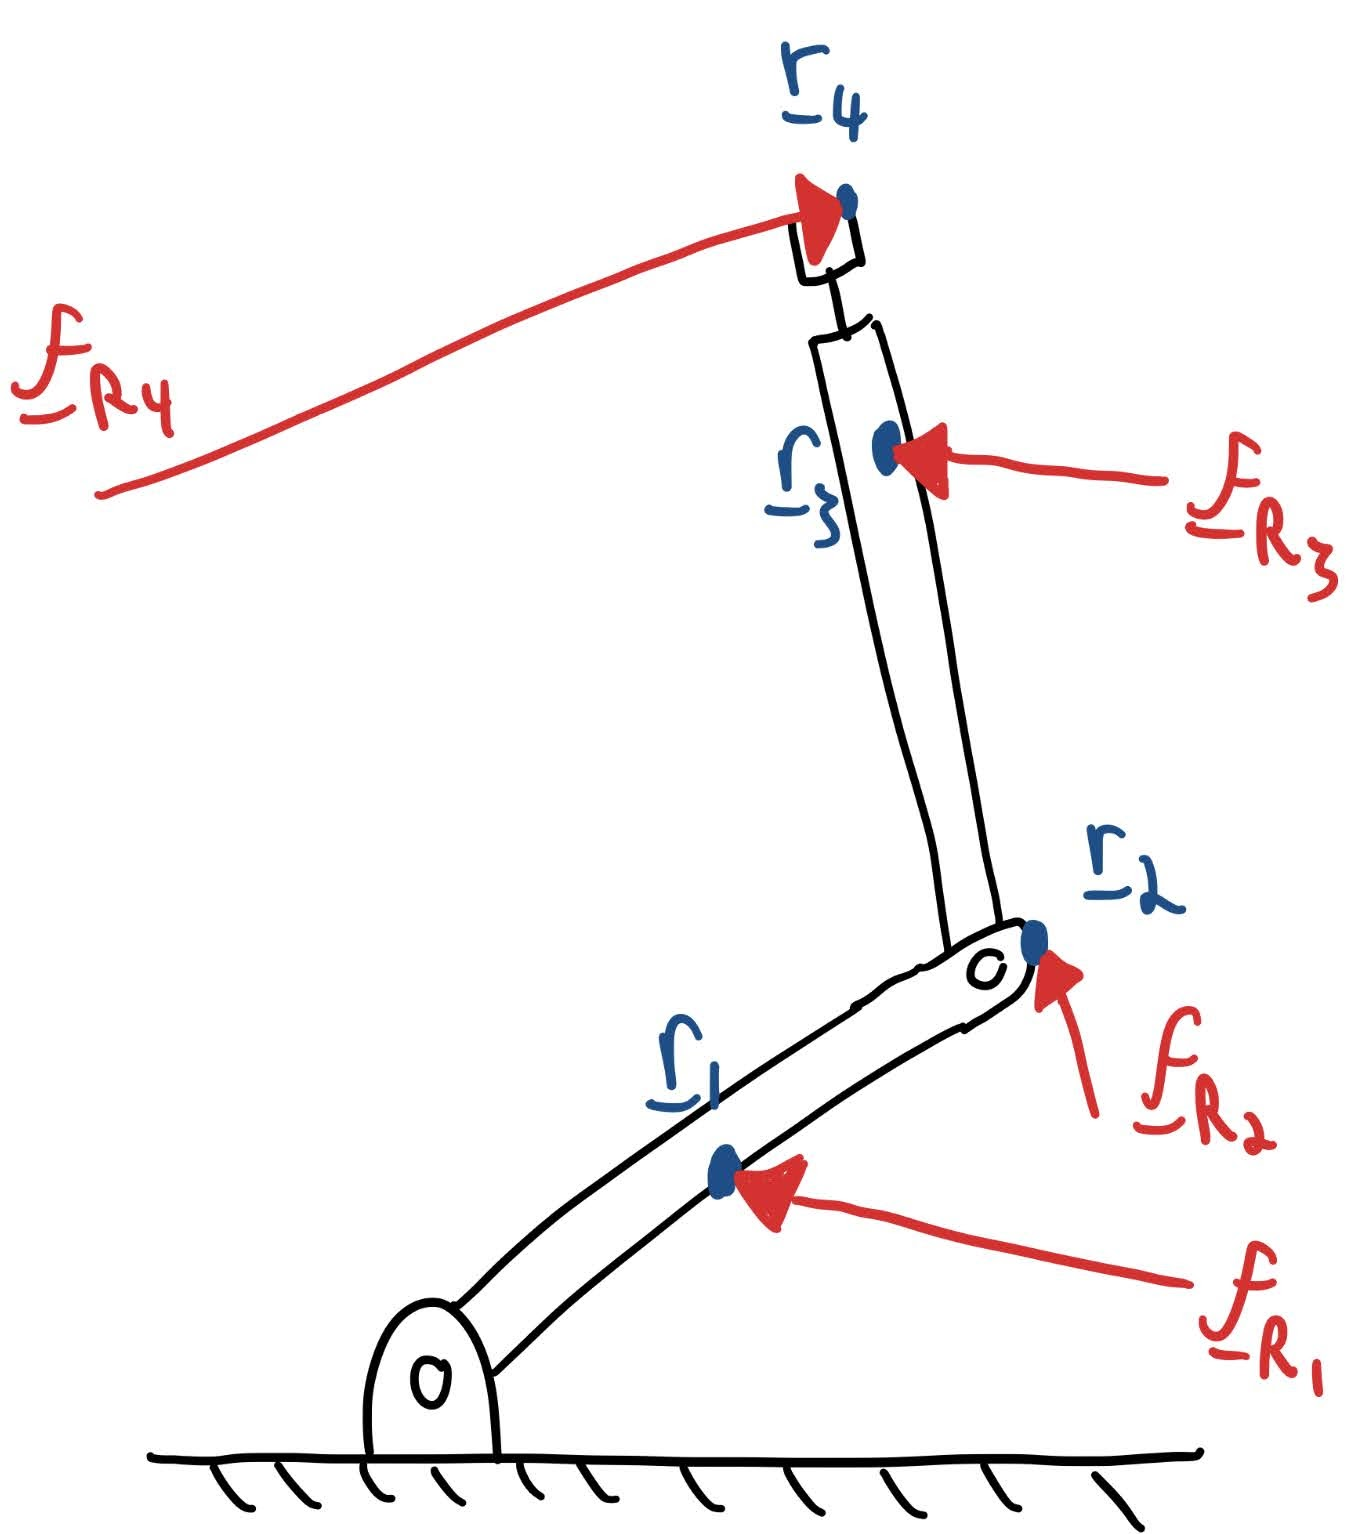
\includegraphics[width=0.40\textwidth]{fig/multipleexternalforces.jpg}
	\caption{Robot avec plusieurs forces externes}%
	\label{fig:multipleexternalforces}
\end{figure}
%%%%%%%%%%%%%%%%%%%%%%%%%%%%%%%%%%%%%%%%%%%%%%%%%%%%%%%%%%%%%%%%%%%%%%%%%%%%





%%%%%%%%%%%%%%%%%%%%%%%%%%%%%%%%%%%%%%%%%%%%%%%%%%%%%%%%%%%
\subsection{Matrice des actionneurs}

La matrice $B(q)$ est une matrice de transformation qui relie le vecteur $\col{u}$,  représentants les entrées du système, et les forces généralisées $\col{\tau}$ associées dans le systèmes de coordonnées $\col{q}$ utilisé pour décrire les équations dans l'espace de la tache:
%%%%%%%%%%%%%%%%%%%%%%%%%%%%%
\begin{align}
\col{\tau} =  B(\col{q})  \col{u} 
\end{align}
%%%%%%%%%%%%%%%%%%%%%%%%%%%%%

\note{Note:}{Dans le chapitre sur la statique (\ref{sec:static}), les divers équations et analyses étaient présentés en assumant qu'on nos actionneurs permettent de commander le vecteur $\col{\tau}$ directement. Ici dans ce chapitre nous incluons une matrice de transformation $B$ pour avoir une représentation plus englobante.}

La Figure \ref{fig:actuatormatrix} illustre qualitativement divers architecture d'actionneurs qui mène à différentes structures pour $B$. Le cas le plus simple est lorsque les entrées $\tau$ sont des forces colocalisées avec les coordonnées généralisées $\col{q}$, par exemple si $\col{u}$ représente des couples net aux joint d'un système alors la matrice $B$ est la matrice identité car les entrée $\col{u}$ sont directement des forces généralisée aux joints $\col{\tau}$. Si on désire que les entrée $\col{u}$ soit directement les couples des moteurs électriques d'un robot alors la matrice $B$ va représenter les ratios de réduction des actionneurs. Ensuite, si les actionneurs ne sont pas colocalisés avec les coordonnées généralisée, alors la matrice $B$ fait le pont entre les forces aux actionneurs et les forces généralisées qu'ils génèrent. Finalement, si il y a moins d'actionneurs que de DDL alors la matrice $B$ ne sera pas carrée. 
%%%%%%%%%%%%%%%%%%%%%%%%%%%%%%%%%%%%%%%%%%%%%%%%%%%%%%%%%%%%%%%%%%%%%%%%%%%%
\begin{figure}[ht]
	\centering
		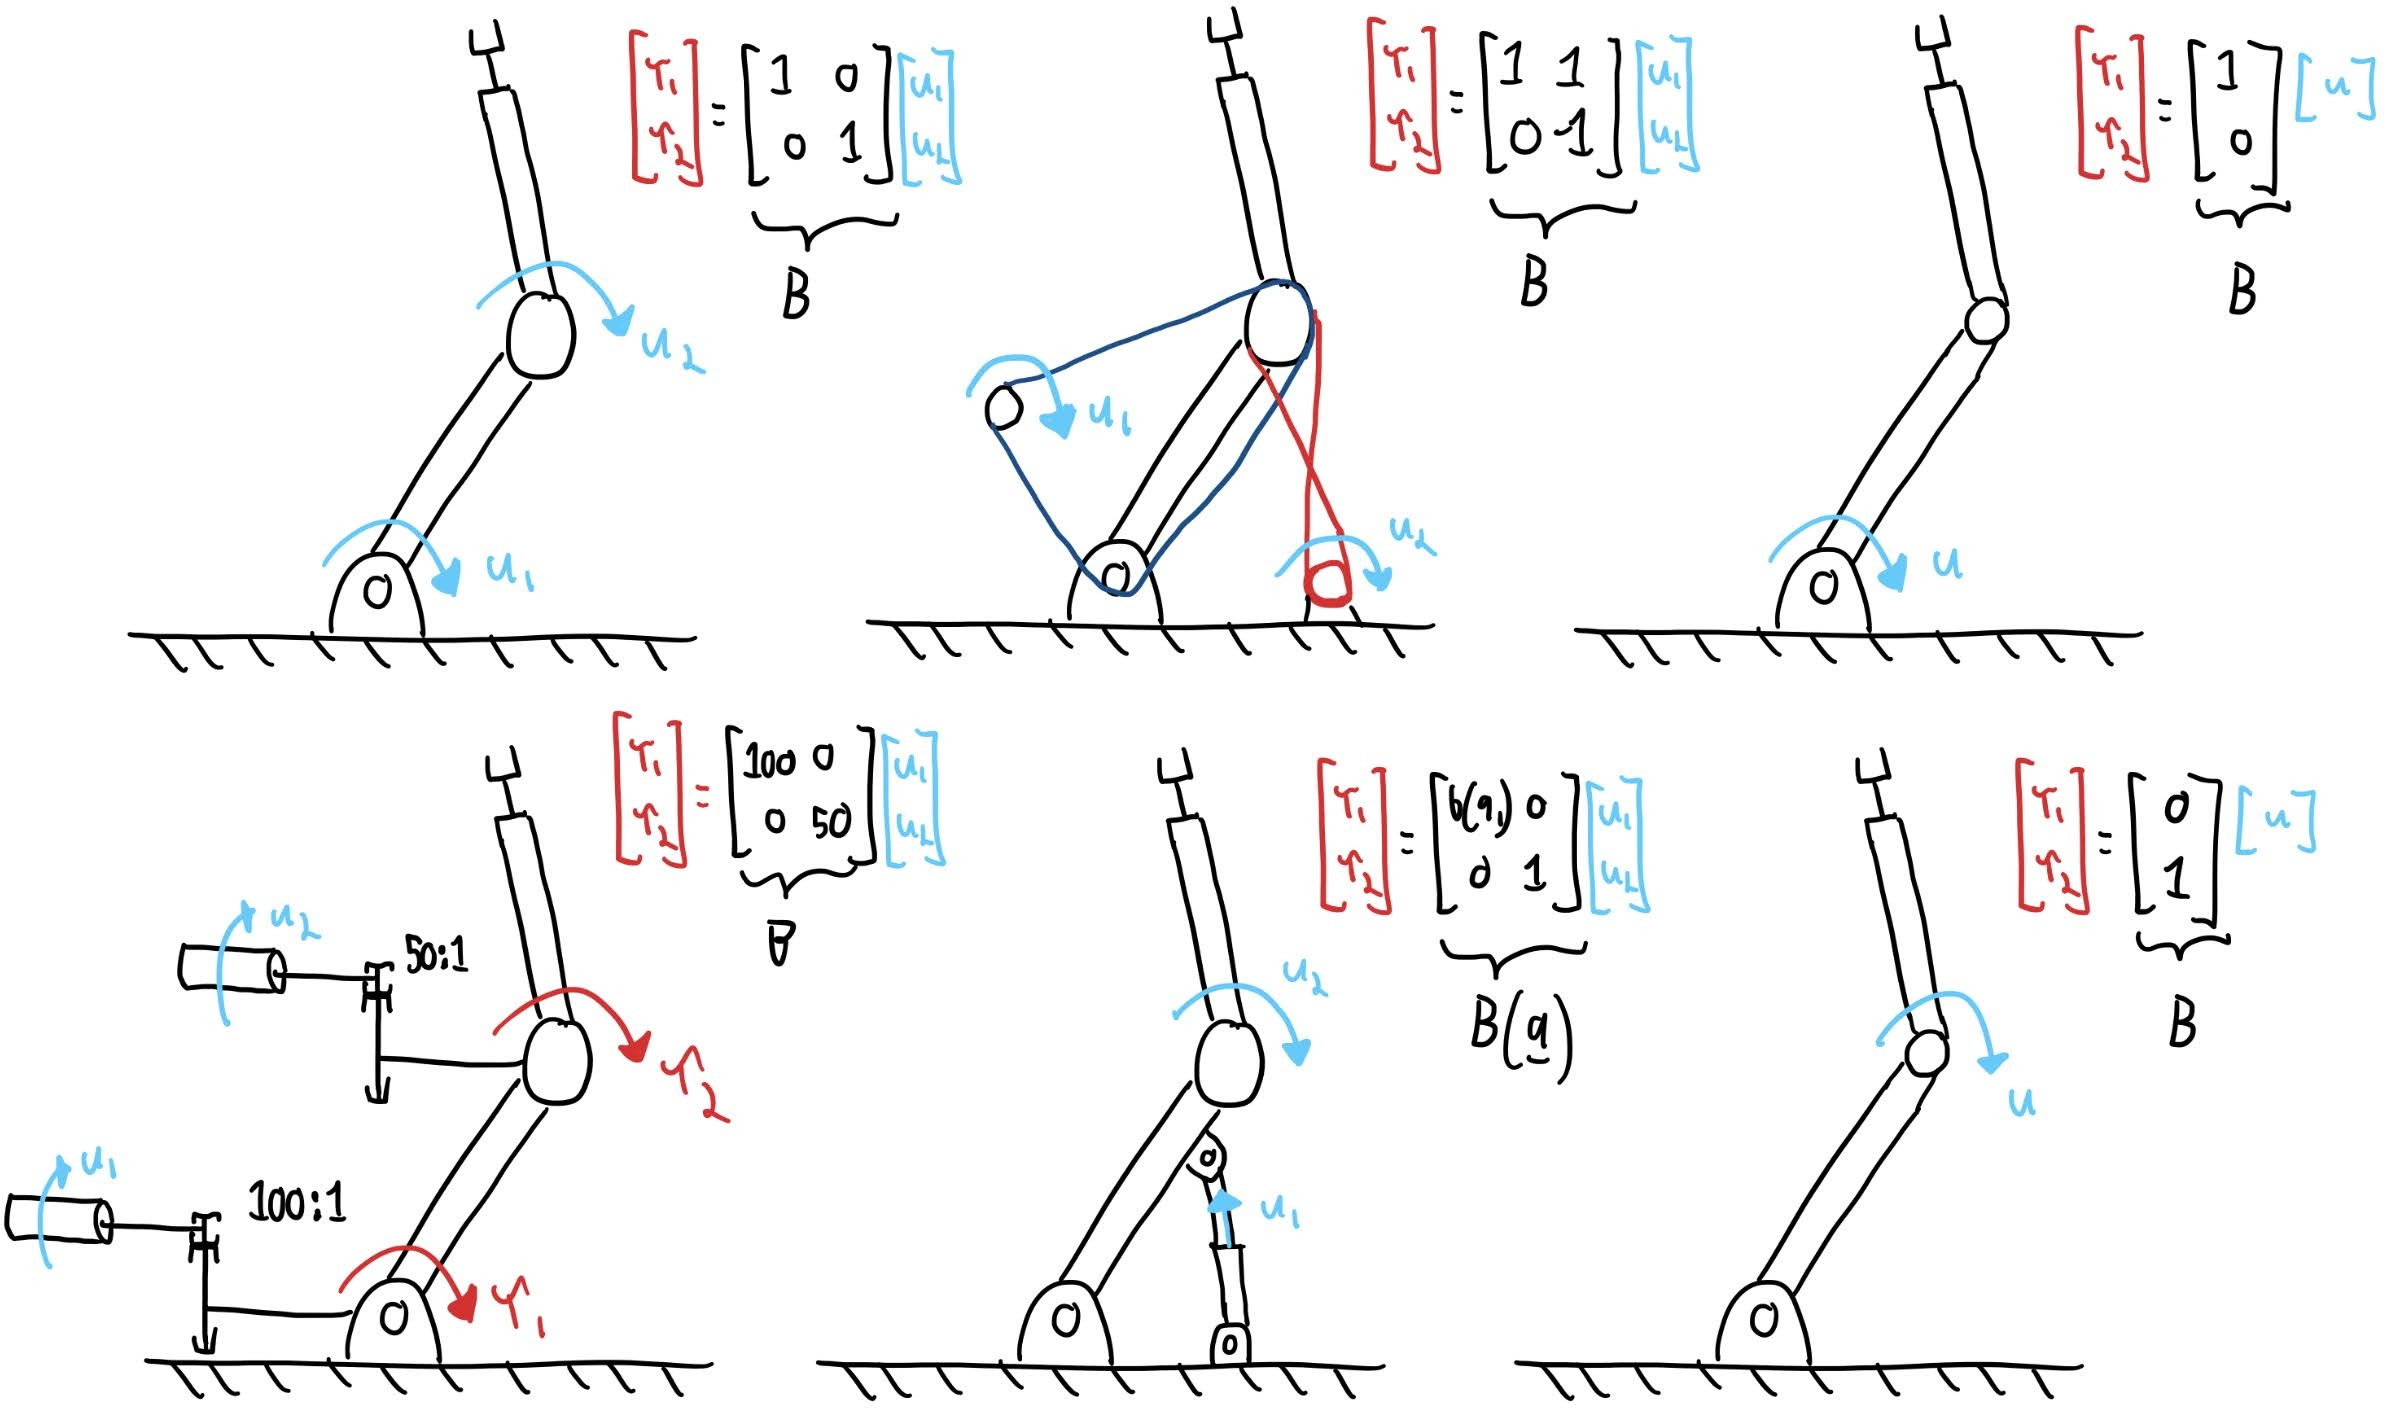
\includegraphics[width=0.99\textwidth]{fig/actuatormatrix.jpg}
	\caption{Matrice $B$ des actionneurs}%
	\label{fig:actuatormatrix}
\end{figure}
%%%%%%%%%%%%%%%%%%%%%%%%%%%%%%%%%%%%%%%%%%%%%%%%%%%%%%%%%%%%%%%%%%%%%%%%%%%%

La notion de puissance est utile pour définir cette matrice: le produit scalaire entre le vecteur vitesse des coordonnées généralisée $\col{\dot{q}}$ et les forces généralisées associées aux actionneurs $B\col{\tau}$ correspond à la puissance entrante fournit par les actionneurs:
%%%%%%%%%%%%%%%%%%%%%%%%%%%%%
\begin{align}
P_{actionneur} = \col{\dot{q}}^T \col{\tau} = \col{\dot{q}}^T B(\col{q}) \col{u}
\end{align}
%%%%%%%%%%%%%%%%%%%%%%%%%%%%%


%%%%%%%%%%%%%%%%%%%%%%%%%%%%%%%%%%%%%%%%%%%%%%%%%%%%%%%%%%%%%%%%%%%%%%%%%%%%
\subsection{Forces conservatrices}

Le vecteur de force conservatrice est défini comme le gradient de l'énergie potentiel par rapport au vecteur de coordonnées généralisée:
%%%%%%%%%%%%%%%%
\begin{align}
 \col{g} ( \col{q} ) = 
\frac{ \partial V(\col{q} ) }{\partial \col{q}^T } 
\end{align}
%%%%%%%%%%%%%%%
de sorte que le taux de variation de l'énergie potentiel soit donnée par
%%%%%%%%%%%%%%%%
\begin{align}
\dot{V} = \frac{\partial V}{ \partial \col{q}} \, \col{\dot{q}} =  \col{g}^T \col{\dot{q}}
\end{align}
%%%%%%%%%%%%%%%%
voir section \ref{sec:manipstaticconservative} pour le détail. 


\textbf{Gravité:} Dans ce chapitre ce vecteur est noté $\col{g}$ car typiquement la seule énergie potentielle significative est l'énergie gravitationnelle et les forces conservatrices sont les forces gravitationnelles. L'énergie potentielle gravitationnelle peut être calculé comme la sommation de l'énergie potentielle de chacun des liens rigides du robot:
%%%%%%%%%%%%%%%%
\begin{align}
V_g(\col{q}) = \sum_i m_i g h_i(\col{q})
\end{align}
%%%%%%%%%%%%%%%
où $m_i$ est la masse du lien $i$, $g$ la constante gravitationnelle et $h_i(\col{q})$ est la hauteur du centre de gravité (c.g.) du lien $i$ exprimée en fonction des coordonnées généralisées, comme illustré à la Figure \ref{fig:gravitycg}. Il est à noter qu'on doit généralement introduire des paramètres géométriques additionnel pour décrire la position des c.g., ici notés avec l'indice $c$.

%%%%%%%%%%%%%%%%%%%%%%%%%%%%%%%%%%%%%%%%%%%%%%%%%%%%%%%%%%%%%%%%%%%%%%%%%%%%
\begin{figure}[ht]
	\centering
		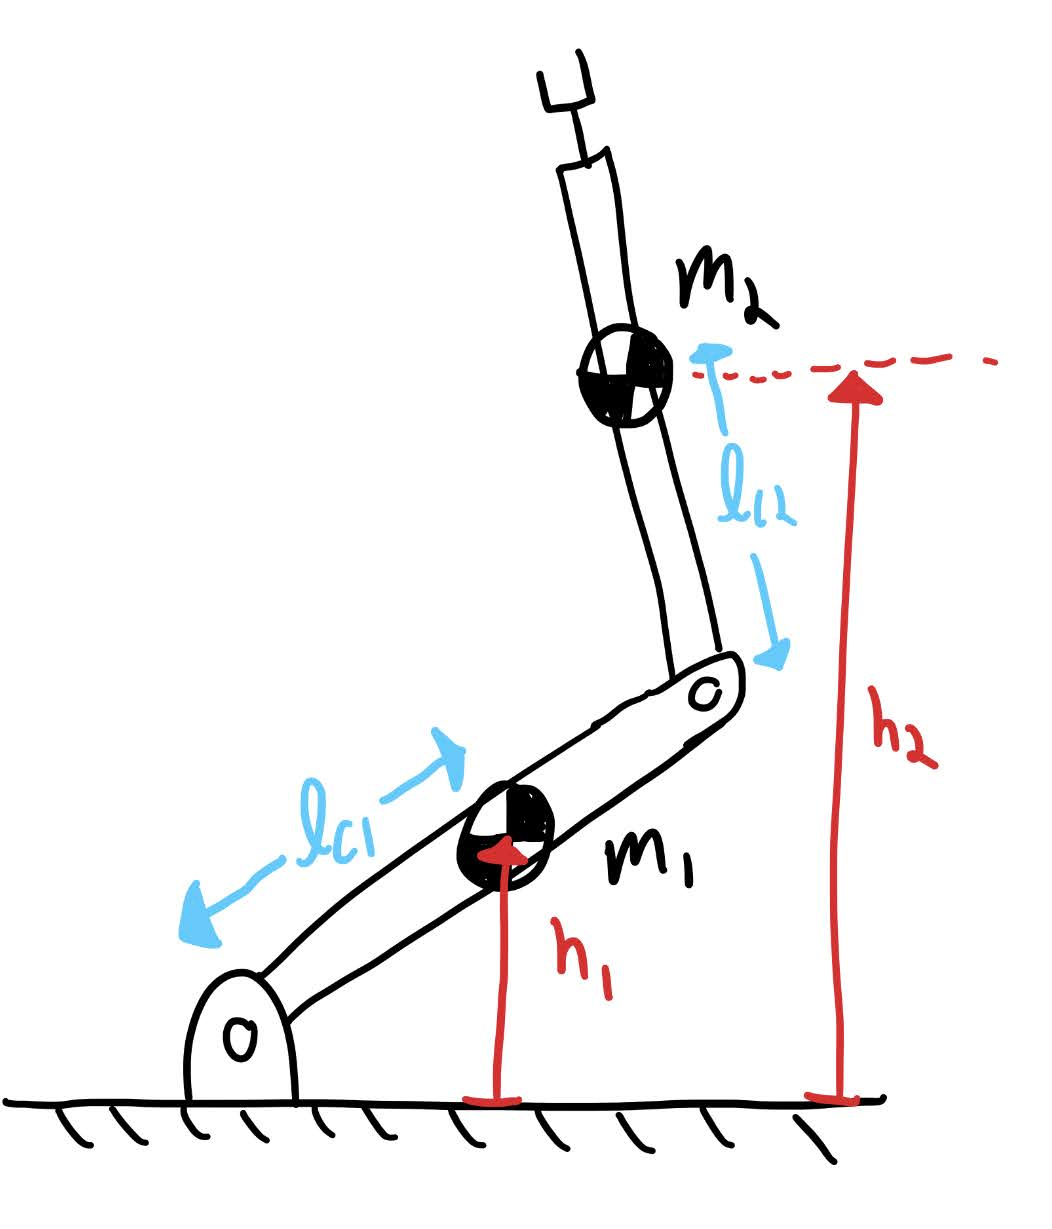
\includegraphics[width=0.50\textwidth]{fig/gravitycg.jpg}
	\caption{La hauteur des centres de gravité des liens rigides}%
	\label{fig:gravitycg}
\end{figure}
%%%%%%%%%%%%%%%%%%%%%%%%%%%%%%%%%%%%%%%%%%%%%%%%%%%%%%%%%%%%%%%%%%%%%%%%%%%%



\newpage
%%%%%%%%%%%%%%%%%%%%%%%%%%%%%%%%%%%%%%%%%%%%%%%%%%%%%%%%%%%%%%%%%%%%%%%%%
\subsection{Forces dissipatrices}

Les forces dissipatrices représentent les phénomènes qui transforment l'énergie du mouvement mécaniques en pertes thermiques et phénomènes irréversibles. Pour être incluse dans l'équation des manipulateurs, ces force doivent être exprimée comme des forces associées aux coordonnées généralisée de sorte que le puissance dissipée soit égale au produit scalaire entre le vecteur de ces forces et le vecteur vitesse:
%%%%%%%%%%%%%%%%
\begin{align}
\dot{Q}_{out} = \dot{\col{q}}^T \col{d}
\end{align}
%%%%%%%%%%%%%%%%

Pour les robots manipulateurs, la principale source de dissipation vient des joints et des actionneurs, ce qui amène généralement à faire l'hypothèse que la force de dissipation $d_i$ est seulement un fonction de la vitesse du joint associé $\dot{q}_i$:
%%%%%%%%%%%%%%%%
\begin{align}
d_i = f_d( \dot{q}_i ) \approx b_s \sgn{(\dot{q}_i)} + b_v \dot{q}_i + \frac{1}{2}\rho C_d A \sgn{(\dot{q}_i)} \dot{q}_i^2
\end{align}
%%%%%%%%%%%%%%%%
Modéliser les phénomènes complexes de friction est une science imparfaite, c'est généralement l'aspect du modèle dynamique d'un robot qui est le moins précis et qui limite la fidélité du modèle. Selon l'objectif de modélisation il va y avoir un compromis à faire entre simplicité et fidélité. Dans un contexte de conception, analyse et/ou développement de loi de commande, on se contente normalement d'approximer la friction comme une combinaison de friction sèche, friction visceuse et friction quadratique, voir Figure \ref{fig:frictionmodels}, mais c'est une grosse approximation de phénomène microscopique de contact complexes. Comme illustré à la Figure \ref{fig:frictionreal}, le comportement observé réel serait typiquement plus complexe et caractérisé par de l'hystérésis.
%%%%%%%%%%%%%%%%%%%%%%%%%%%%%%%%%%%%%%%%%%%%%%%%%%%%%%%%%%%%%%%%%%%%%%%%%%%%
\begin{figure}[ht]
	\centering
		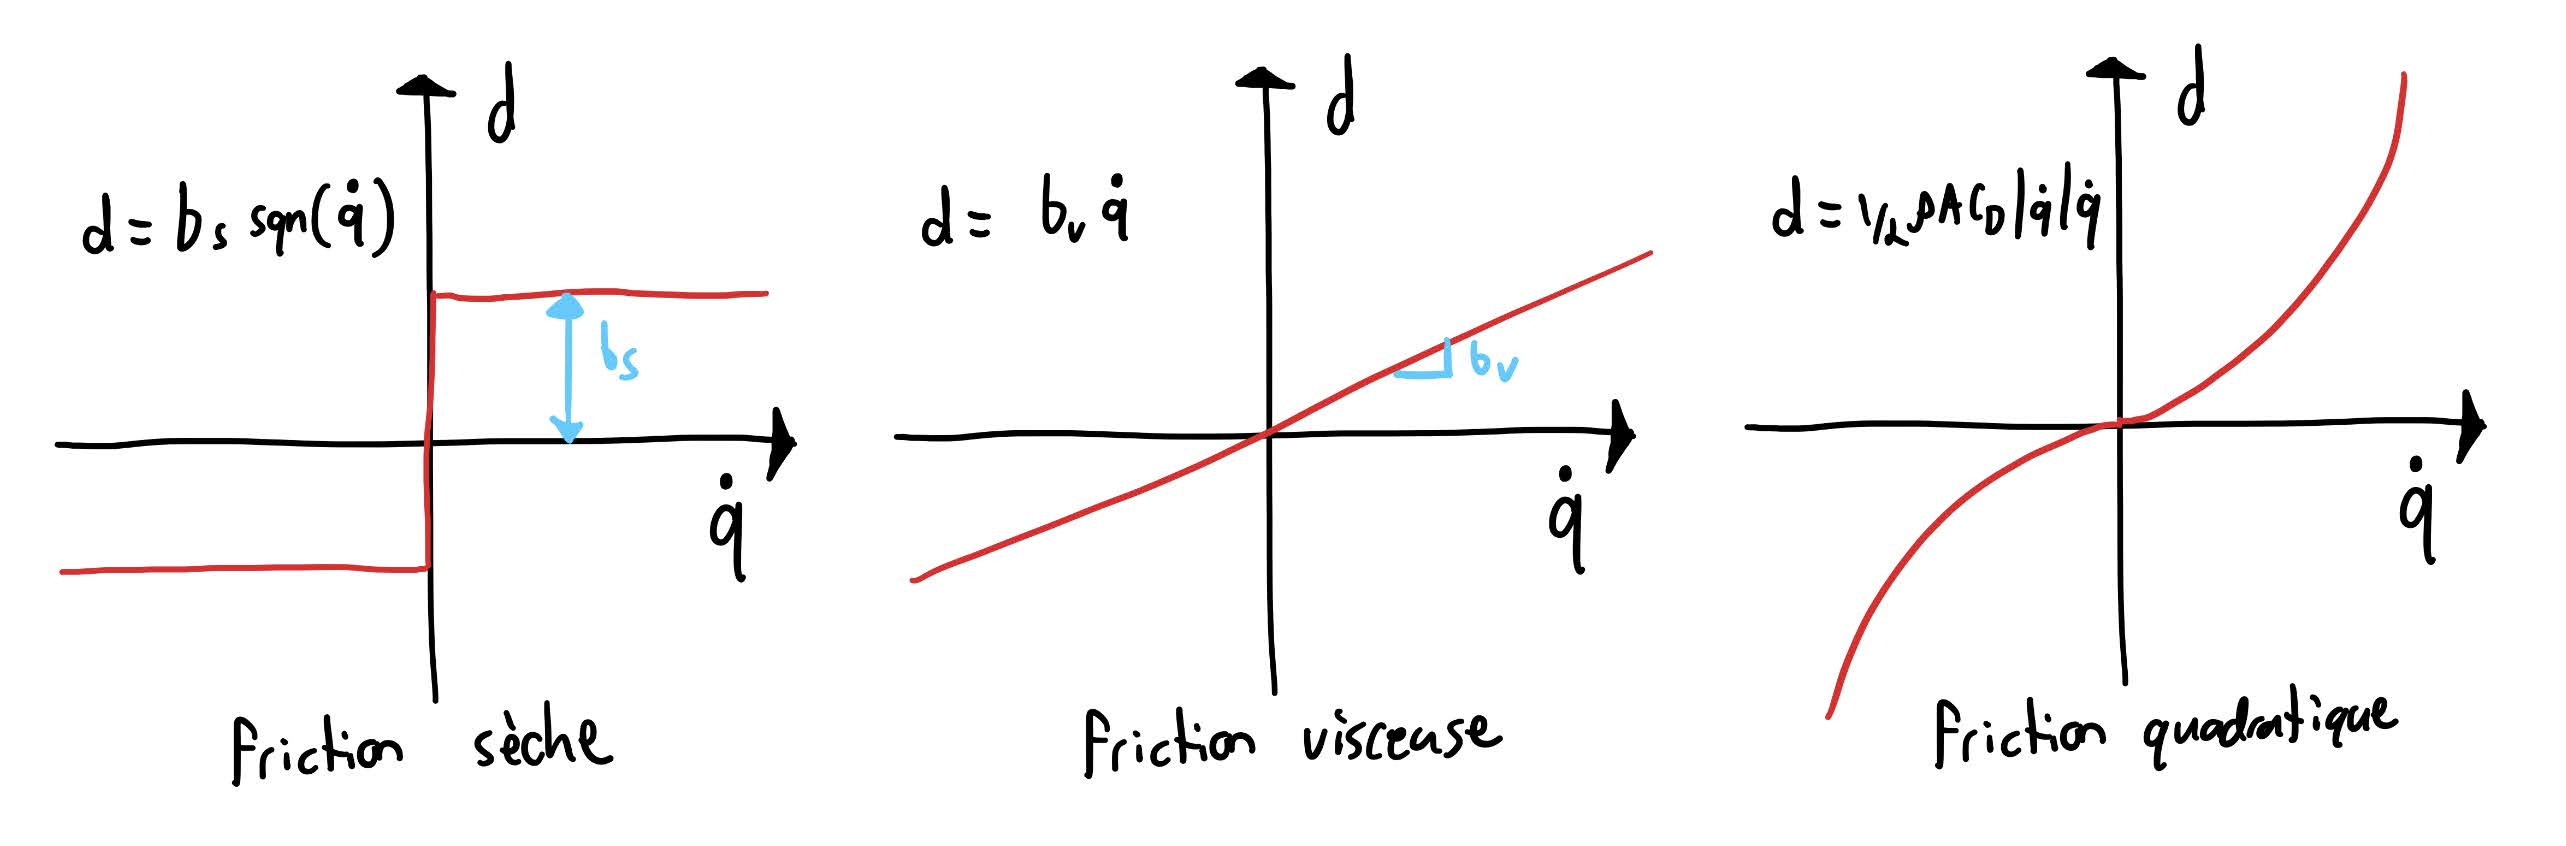
\includegraphics[width=0.99\textwidth]{fig/frictionmodels.jpg}
	\caption{Modèles simples de friction}%
	\label{fig:frictionmodels}
\end{figure}
%%%%%%%%%%%%%%%%%%%%%%%%%%%%%%%%%%%%%%%%%%%%%%%%%%%%%%%%%%%%%%%%%%%%%%%%%%%%

%%%%%%%%%%%%%%%%%%%%%%%%%%%%%%%%%%%%%%%%%%%%%%%%%%%%%%%%%%%%%%%%%%%%%%%%%%%%
\begin{figure}[ht]
	\centering
		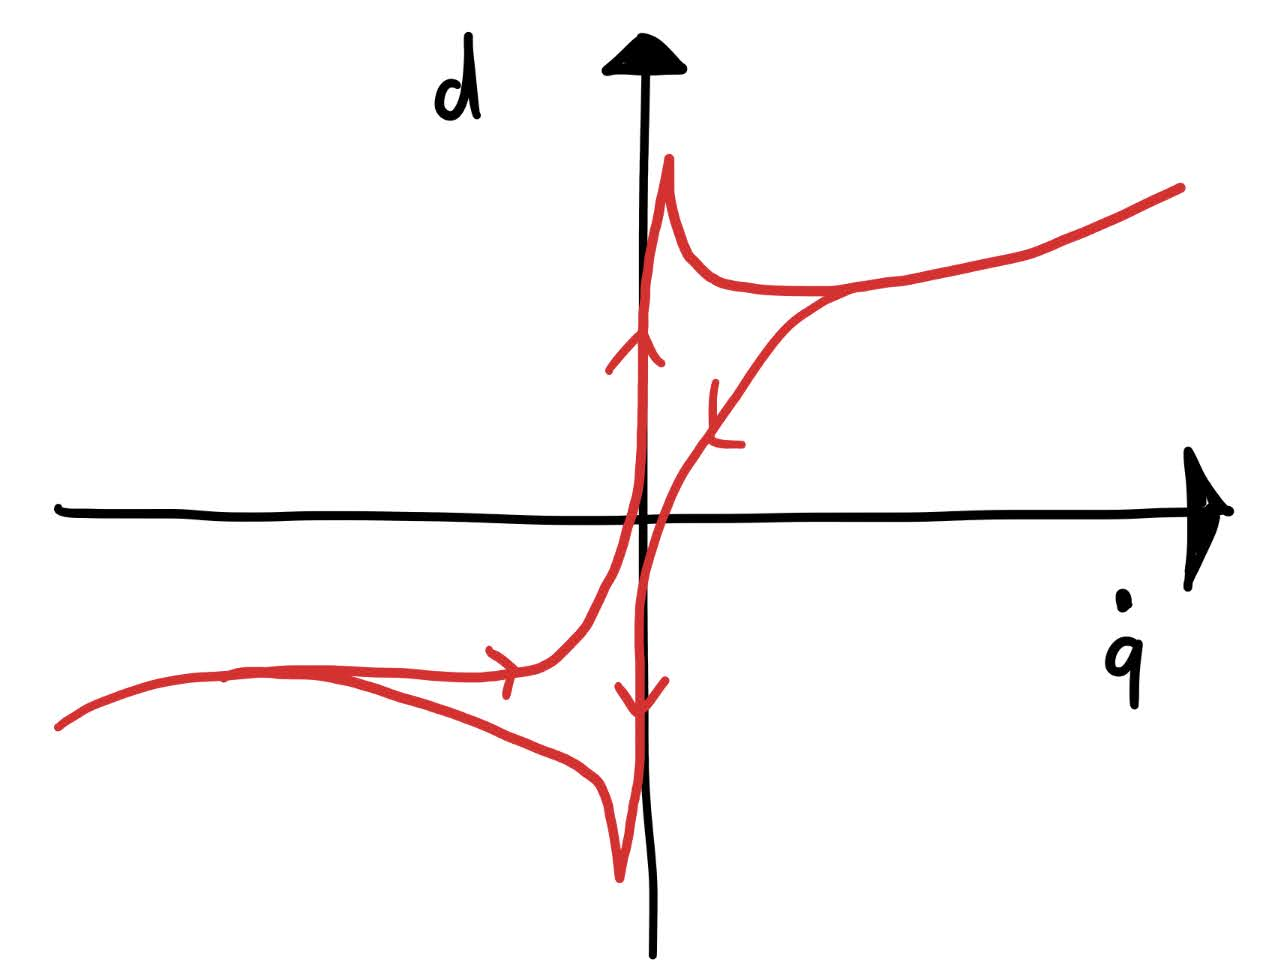
\includegraphics[width=0.40\textwidth]{fig/frictionreal.jpg}
	\caption{Friction: comportement réel}%
	\label{fig:frictionreal}
\end{figure}
%%%%%%%%%%%%%%%%%%%%%%%%%%%%%%%%%%%%%%%%%%%%%%%%%%%%%%%%%%%%%%%%%%%%%%%%%%%%


\newpage
%%%%%%%%%%%%%%%%%%%%%%%%%%%%%%%%%%%%%%%%%%%%%%%%%%%%%%%%%%%%%%%%%%%%%%%%%%%%
\subsection{Effets inertiels}
%

Les termes $H(\col{q}) \col{\ddot{q}}$ et $C(\col{q},\col{\dot{q}})\col{\dot{q}}$ dans l'équation des manipulateur sont l'équivalent du terme $ma$ dans l'équation $f=ma$ alors que tout les autres termes sont des forces. Ici le terme $ma$ prend cette forme particulière car il est exprimé dans les coordonnées généralisée du système relié à l'espace des joints. Le terme $H(\col{q}) \col{\ddot{q}}$ représente la "force" inertielle nécessaire pour obtenir une accélération $\col{\ddot{q}}$ à un configuration $\col{q}$, alors que le terme $C(\col{q},\col{\dot{q}})$ représente une "force" inertielle nécessaire pour maintenir une certaine vitesse $\col{\dot{q}}$ à la configuration $\col{q}$, comme l'effet centrifuge ou de coriolis. Le second terme existe seulement lorsque la matrice $H$ varie dans le temps, lorsque de momentum peut varier sans avoir une variation de vitesse dans l'espace des joints. 

\subsubsection{Energie cinétique: }
L'énergie cinétique $T$ du système est directement reliée à la matrice d'inertie $H$ et la vitesse des joints $\dot{\col{q}}$. L'équivalent multi-dimension de l'équation de l'énergie cinémique scalaire $\frac{1}{2}mv^2$ est donné par:
%%%%%%%%%%%%%%%%%%%%
\begin{align}
T(\col{q},\col{\dot{q}}) = \frac{1}{2} \col{\dot{q}}^T H(\col{q}) \col{\dot{q}}  =
\frac{1}{2} \sum_i \sum_j H_{ij} \dot{q}_i \dot{q}_j
\label{eq:kinetic}
\end{align}
%%%%%%%%%%%%%%%%%%%%
\note{Propriété de la matrice $H$: }{Il est a noté que la matrice d'inertie est une matrice $n$ x $n$ ($n$ est le nombre de DDL), toujours symétrique et définie positive (ce qui veux dire que l'équation ci-dessus ne peut jamais prendre de valeur négative peut importe le vecteur vitesse $\col{\dot{q}}$). Cela implique que l'inverse $H^{-1}$ va toujours exister, une propriété qui sera utile pour la suite!}

La matrice $C$, souvent appelé la matrice de coriolis, n'est pas une propriété indépendante du système, elle est en fait reliée à la variation temporelle de la matrice $H$:
%%%%%%%%%%%%%%%%%%%%
\begin{align}
\dot{H} = C + C^T
\label{eq:cener}
\end{align}
%%%%%%%%%%%%%%%%%%%%
On peut en fait aussi définir directement la matrice $C$ connaissant l'expression de la matrice $H$ en utilisant la relation suivante:
%%%%%%%%%%%%%%%%%%%%
\begin{align}
C_{ij} = \sum_k \Gamma_{ijk} \dot{q}_k \quad \text{avec} \quad \Gamma_{ijk} = \frac{1}{2}\left(  \frac{\partial H_{ij}}{\partial q_k} + \frac{\partial H_{ik}}{\partial q_j} - \frac{\partial H_{jk}}{\partial q_i}   \right)
\end{align}
%%%%%%%%%%%%%%%%%%%%
Si on définie $\col{c}$ comme le vecteur résultant du terme $C(\col{q},\col{\dot{q}})\col{\dot{q}}$, on peut aussi obtenir la relation sous cette forme:
%%%%%%%%%%%%%%%%%%%%
\begin{align}
c_i &= \sum_j \sum_k \Gamma_{ijk} \dot{q}_j \dot{q}_k \\ 
\col{c} &= C(\col{q},\col{\dot{q}})\col{\dot{q}} = \col{\dot{q}}^T \Gamma(\col{q}) \col{\dot{q}}
\end{align}
%%%%%%%%%%%%%%%%%%%%

\begin{proof}
À venir!! voir photo ipad alex 26 janvier 2023
\end{proof}

%
% TODO la version indicielle

%\subsubsection{Momentum:}
%Le momentum du système serait ici une quantitée vectorielle donnée par:
%%%%%%%%%%%%%%%%%%%%
%\begin{align}
%\col{p} = H(\col{q}) \col{\dot{q}}
%\end{align}
%%%%%%%%%%%%%%%%%%%%

\newpage
%%%%%%%%%%%%%%%%%%%%%%%%%%%%%%%%%%%%%%%%%%%%%%%%%%%%%%%%%%%
\subsection{Forme compacte des équations des manipulateurs}

Parfois pour allégé la manipulation des équations, une version abrégée où $\col{c}$ est parfois utilisé pour regrouper toute les forces internes (qui sont des fonctions des états du systèmes):
%%%%%%%%%%%%%%%%%%%%%%%
\begin{align}
\col{h} = C(\col{q},\col{\dot{q}}) \col{\dot{q}} + d(\col{q}, \col{\dot{q}}) + \col{g}(\col{q})
\end{align}
%%%%%%%%%%%%%%%%%%%%%%%
ce qui simplifie, pour un cas sans forces externes, l'équation des manipulateurs à:
%%%%%%%%%%%%%%%%%%%%%%%
\begin{align}
H \col{\ddot{q}} + \col{h} = \col{\tau} 
\label{eq:manipulator_short}
\end{align}
%%%%%%%%%%%%%%%%%%%%%%%


%\newpage
%%%%%%%%%%%%%%%%%%%%%%%%%%%%%%%%%%%%%%%%%%%%%%%%%%%%%%%%%%%
\subsection{Systèmes de coordonnées additionnels}
\label{sec:coord}
%%%%%%%%%%%%%%%%%%%%%%%%%%%%%%%%%%%%%%%%%%%%%%%%%%%%%%%%%%%

TODO: Uniformiser le nom des variables pour cette section.

\newline
Parfois il peut être utile de travailler avec des systèmes de coordonnées supplémentaire à l'espace des joints. La Figure \ref{fig:coord} montre quelques espaces supplémentaires qui peuvent être utilisés. 
%
\begin{figure}[H]
	\centering
		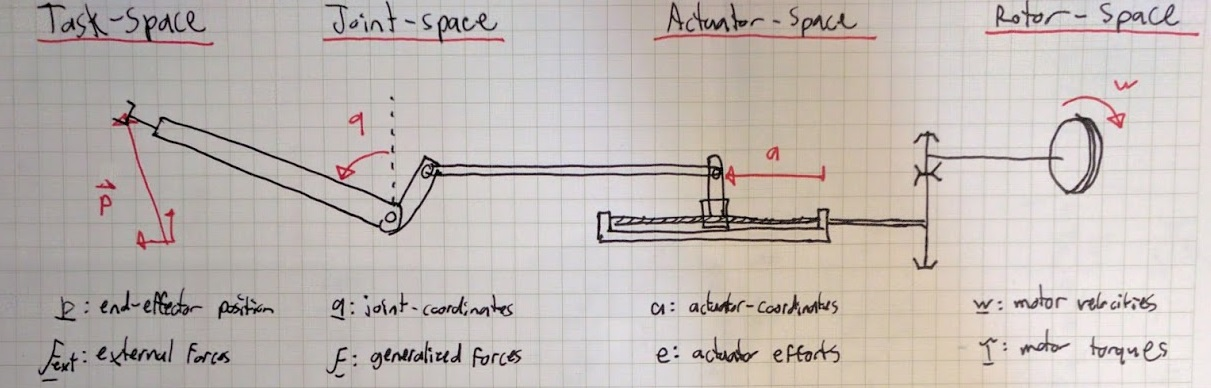
\includegraphics[width=0.99\textwidth]{coord.jpg}
	\caption{Coordinate systems}%
	\label{fig:coord}
\end{figure}
%
Si les relations cinématiques entre les coordonnées de ces espaces sont donné par:
%
\begin{align}
\col{\dot{r}}   &= J_e( \col{q} ) \col{\dot{q} }  \quad \text{ de l'espace des joints vers l'espace de la tâche   } \\
\col{\dot{a}}   &= J_a( \col{q} ) \col{\dot{q} }  \quad \text{ de l'espace des joints vers l'espace des actionneurs } \\
\col{w }        &= R              \col{\dot{a} }  \quad\quad \text{ de l'espace des actionneurs vers l'espace des moteurs } 
\label{eq:coord_transform2}
\end{align}
%
%
On pourrait utiliser ces relations pour inclure directement des forces dans l'espace des actionneurs $\col{f}_a$, et définir $\col{\tau}$ comme les couples moteurs plutôt celui rapporté au joint ainsi:
%%%%%%%%%%%%%%%%%%%%%%%%%%%%%
\begin{align}
H \col{\ddot{q}} + C \col{\dot{q}} + \col{d} + \col{g} =  \underbrace{ J_a^T(\col{q}) R^T }_{B(\col{q})}  \col{u} + J_e^T(\col{q}) \col{f}_e + J_a^T(\col{q}) \col{f}_a
\label{eq:manipulator_gen}
\end{align}
%%%%%%%%%%%%%%%%%%%%%%%%%%%%%


\newpage
%%%%%%%%%%%%%%%%%%%%%%%%%%%%%%%%%%%%%%%%%%%%%%%%%%%%%%%%%%%
\section{Conservation de l'énergie}
%%%%%%%%%%%%%%%%%%%%%%%%%%%%%%%%%%%%%%%%%%%%%%%%%%%%%%%%%%%

Si on reprend le bilan d'énergie avec le volume de contrôle de la figure \ref{fig:controlvolume}, mais cette fois çi en incluant aussi l'énergie cinétique dans l'énergie interne $E$ et les pertes thermiques dues aux forces dissipatrices $\dot{Q}$, on trouve avec la première loi de la thermodynamique:
%%%%%%%%%%%%%%%%%%%%%%%%%%%%%
\begin{align}
\frac{dE}{dt}     &= P_{in} - P_{out} \\
\dot{T} + \dot{V}  &= \sum \tau_i \dot{q}_i  - \sum f_i \dot{r}_i - \dot{Q} \\
\frac{d}{dt}\left( \frac{1}{2} \col{\dot{q}}^T H \col{\dot{q}} \right) + \frac{\partial V}{\partial \col{q}^T} \dot{\col{q}} &= \col{\tau}^T \col{\dot{q}}  - \col{f}_E^T J \col{\dot{q}} - \col{d}^T \col{\dot{q}} \\
\dot{\col{q}}^T H \col{\ddot{q}} + \dot{\col{q}}^T \frac{1}{2}\dot{H}\dot{\col{q}} + \dot{\col{q}}^T \col{g} &=  \dot{\col{q}}^T B\col{u} + \dot{\col{q}}^T J^T \col{f}_{R_E}  - \dot{\col{q}}^T \col{d}
\end{align}
%%%%%%%%%%%%%%%%%%%%%%%%%%%%%

On peut donc voir toute l'expression comme un produit scalaire entre le vecteur et les termes restant qui peuvent être simplifier si on substitue par notre définition de l'équation des manipulateurs. Les seules termes qui ne s'annulent pas sont $\dot{H}$ et $C$, ce qui mène à une relation entre les deux:
%%%%%%%%%%%%%%%%%%%%%%%%%%%%%
\begin{align}
\dot{\col{q}}^T \left[ H \col{\ddot{q}} + \frac{1}{2}\dot{H}\dot{\col{q}} + \col{g} + \col{d} - \col{\tau} - J^T \col{f}_E  \right] &= 0 \\
\dot{\col{q}}^T \left[ \frac{1}{2}\dot{H} - C \right] \dot{\col{q}} &= 0
\end{align}
%%%%%%%%%%%%%%%%%%%%%%%%%%%%%
Cette expression va toujours être égale à zéro si $\dot{H} = C + C^T$, une condition qui correspond donc d'un certain sens à une condition pour la conservation de l'énergie pour le système.

\note{Matrice anti-symétrique}{Une matrice est dit anti-symétrique, \textit{skew-symetric }en anglais, si ...}

%\newpage
%%%%%%%%%%%%%%%%%%%%%%%%%%%%%%%%%%%%%%%%%%%%%%%%%%%%%%%%%%%
\section{Dynamique inverse}
\label{sec:inversedynamic}
%%%%%%%%%%%%%%%%%%%%%%%%%%%%%%%%%%%%%%%%%%%%%%%%%%%%%%%%%%%

L'équation des manipulateurs détermine des forces généralisée $\col{\tau}$ pour une configuration $\col{q}$, une vitesse $\col{\dot{q}}$ et une accélération $\col{\ddot{q}}$. La dynamique inverse représente la même équation mais lorsqu'on isole le vecteur accélération comme une fonction de toute les forces internes et externes, c'est en fait le seul normal de la causalité. En version compacte on peut retrouver:
%%%%%%%%%%%%%%%%%%%%%%%
\begin{align}
\col{\ddot{q}}  = H^{-1} \left( \col{\tau} - \col{h} \right)
\end{align}
%%%%%%%%%%%%%%%%%%%%%%%
ou en version longue:
%%%%%%%%%%%%%%%%%%%%%%%
\begin{align}
\col{\ddot{q}}  = H^{-1}(\col{q}) \left( B(\col{q}) \col{u}  + J^T(\col{q}) \col{f}_{R_E} - C(\col{q},\col{\dot{q}}) \col{\dot{q}} - d(\col{q}, \col{\dot{q}}) - \col{g}(\col{q})  \right)
\end{align}
%%%%%%%%%%%%%%%%%%%%%%%
Comme la matrice d'inertie $H$ est symétrique et définie positive, sont inverse existe toujours et donc cette équation a toujours une solution.

%\newpage
%%%%%%%%%%%%%%%%%%%%%%%%%%%%%%%%%%%%%%%%%%%%%%%%%%%%%%%%%%%
\section{Systèmes sous-actionnés vs. complètement actionnés}
\label{sec:underactuated}
%%%%%%%%%%%%%%%%%%%%%%%%%%%%%%%%%%%%%%%%%%%%%%%%%%%%%%%%%%%

Une caractéristique importante pour déterminer les capabilités physique d'un robot manipulateur est de déterminer si le système est pleinement ou sous-actionné. Un système pleinement actionné a la capacité (théorique) d'imposer un vecteur d'accélération $\col{\ddot{q}}$ arbitraire si on suppose que le vecteur d'entrée $\col{u}$ peut prendre des valeurs arbitraires (pas de maximum ou minimum). La condition mathématique pour être pleinement actionné est que le rang (rangé si la matrice n'est pas carrée) de $B$ doit être égal à $n$, le nombre de DDL. On dira alors que le système est sous-actionné si
%%%%%%%%%%%%%%%%%%%%%%%
\begin{align}
rang\left( B(\col{q}) \right) < n = dim( \col{q} )
\end{align}
%%%%%%%%%%%%%%%%%%%%%%%

%%%%%%%%%%%%%%%%%%%%%%%%%%%%%%%%%%%%%%%%%%%%%%%%%%%%%%%%%%%
\section{Manipulabilité dynamique}
\label{sec:dynamicmanipulability}
%%%%%%%%%%%%%%%%%%%%%%%%%%%%%%%%%%%%%%%%%%%%%%%%%%%%%%%%%%%

À la section \ref{sec:velocitymanipulability}, la notion de manipulabilité définissait une enveloppe de vitesse possible à l'effecteur. Il est aussi possible d'analyser l'enveloppe d'accélérations cartésiennes possibles à l'effecteur pour un vecteur de couple des actionneurs unitaire. 

Détails à venir!



\newpage
%%%%%%%%%%%%%%%%%%%%%%%%%%%%%%%%%%%%%%%%%%%%%%%%%%%%%%%%%%%
\section{Dérivation des équations avec la méthode de Lagrange}
\label{sec:lagrange}
%%%%%%%%%%%%%%%%%%%%%%%%%%%%%%%%%%%%%%%%%%%%%%%%%%%%%%%%%%%

Pour des systèmes robotiques et mécanismes articulés relativement simpleS, la méthode de Lagrange est un outil bien adapté pour calculé rapidement analytiquement les équations du mouvement. Pour utiliser cette méthode, il suffit de déterminer les expressions pour l'énergie cinétique et potentielle en fonction des coordonnées généralisée.:
%%%%%%%%%%%%%%%%
\begin{align}
\mathcal{L} &= T - V = 
\underbrace{T(\col{q},\col{\dot{q}})}_{\text{Énergie cinétique}}
- 
\underbrace{V(\col{q})}_{\text{Énergie potentielle}}
\end{align}
%%%%%%%%%%%%%%%
Ensuite il suffit d'appliquer une "recette de cuisine" qui consiste a effectuer des dérivées pour obtenir les équations de la dynamique. Chaque ligne $i$ de l'équation des manipulateurs peut être déterminée avec l'expression suivante:
%%%%%%%%%%%%%%%%
\begin{align}
\forall i \quad \quad \frac{d}{dt}\left(\frac{\partial \mathcal{L}}{\partial \dot{q}_i}\right) - \frac{\partial \mathcal{L}}{\partial q_i} = \sum \tau_i
\end{align}
%%%%%%%%%%%%%%%
qui est aussi équivalente à:
%%%%%%%%%%%%%%%%
\begin{align}
\forall i \quad \quad 
\underbrace{
\frac{d}{dt}(\frac{\partial T}{\partial \dot{q}_i}) 
- 
\frac{\partial T}{\partial q_i} 
}_{\text{Effets inertiels}}
+
\underbrace{
\frac{\partial V}{\partial q_i} 
}_{\text{Force conservatrices}}
= 
\underbrace{
\sum \tau_i
}_{\text{Forces dissipatrices, externes et actionneurs}}
\end{align}
%%%%%%%%%%%%%%%
On voit donc que cette méthode est surtout intéressante pour déterminer les termes inertiels et les forces conservatives, est ne guide pas vraiment la détermination des autres forces ni leur expression comme des forces généralisées. L'avantage de cette méthode est qu'il est possible d'ignorer les forces de contraintes dans la démarche, versus la méthode classique qui demanderait de débuter par des diagrammes de corps libres (DCL), appliqué $f=ma$ sur tout les axes et faire un processus d'élimination des forces de contrainte. 

\video{Méthode de Lagrange pour déterminer les équations dynamiques}{https://youtu.be/AUcs0L85liM}

\note{Note: }{Il est a noté que la méthode de Lagrange n'est pas un type de modèle mais bien une méthodologie, i.e. une recette de cuisine pour déterminer les équations dynamiques d'un système de corps rigides. En utilisant la méthode classique (DCL + lois de Newtons) ou n'importe quelle autre méthode, si on part des mêmes hypothèses de modélisation on va trouver exactement les mêmes équations.}



\newpage
%%%%%%%%%%%%%%%%%%%%%%%%%%%%%%%%%%%%%%%%%%%%%%%%%%%%%%%%%%%
\section{Équations dans l'espace de la tâche}
\label{sec:taskdynamics}
%%%%%%%%%%%%%%%%%%%%%%%%%%%%%%%%%%%%%%%%%%%%%%%%%%%%%%%%%%%

En dérivant la relation de cinématique différentielle il est possible d'obtenir des relations entre les vitesses et accélérations:
%%%%%%%%%%%%%%%%
\begin{align}
\col{\dot{r}} &= J \col{\dot{q}} \\
\col{\ddot{r}} &= J \col{\ddot{q}}  + \dot{J} \col{\dot{q}} 
\end{align}
%%%%%%%%%%%%%%%
Ensuite si on utilise ces équations pour remplacer les variables de l'espace des joints par ceux dans l'espace de la tâche dans l'équation des manipulateurs:
%%%%%%%%%%%%%%%%
\begin{align}
H \col{\ddot{q}} + \col{c} &= \col{\tau} + J^T \col{f}_{R_E} \\
H J^{-1} (\col{\ddot{r}} - \dot{J} \col{\dot{q}}) + \col{h} &= \col{\tau} + J^T \col{f}_{R_E}
\end{align}
%%%%%%%%%%%%%%%%
et qu'on multiplie ensuite par la droite par l'inverse du jacobien transposé ($J^{-T}=(J^T)^{-1}$), nous obtenons:
%%%%%%%%%%%%%%%%
\begin{align}
J^{-T} H J^{-1} \col{\ddot{r}} -  J^{-T} H J^{-1} \dot{J} \col{\dot{q}} + J^{-T} \col{h} &= J^{-T} B \col{u} + J^{-T} J^T \col{f}_{R_E} \\
\underbrace{
J^{-T} H J^{-1} 
}_{H^r}
\col{\ddot{r}} +  
\underbrace{
J^{-T} \col{h} 
-
J^{-T} H J^{-1} \dot{J} J^{-1} 
\col{\dot{r}} 
}_{\col{h}^r}
&= 
\underbrace{
J^{-T} 
B
}_{B^r}
\col{u} + \col{f}_{R_E} 
\end{align}
%%%%%%%%%%%%%%%%
Nous pouvons ensuite réorganiser les termes pour obtenir une nouvelle équation, qui a la même forme originale que l'équation des manipulateurs dans l'espace des joints, mais avec tout les termes par rapport aux coordonnées de la tâche:
%%%%%%%%%%%%%%%%
\begin{align}
H^r
\col{\ddot{r}} +  
\col{h}^r
&= B^{r} \col{u} + \col{f}_{R_E} 
\end{align}
%%%%%%%%%%%%%%%%
où
%%%%%%%%%%%%%%%%
\begin{align}
H^r & = J^{-T} H J^{-1} \\
\col{h}^r & = J^{-T} \col{h}  - H^r \dot{J} J^{-1} \col{\dot{r}}  \\
B^r & = J^{-T} B
\end{align}
%%%%%%%%%%%%%%%%
Cette équation représente la même dynamique mais exprimée avec les coordonnées de l'espace de la tâche directement. Il est à noter que cette transformation de coordonnées n'est pas possible sur une singularité. Si l'espace de la tâche représente des coordonnées cartésienne de l'outil du robot, alors la matrice $H^r$ représente l'inertie ressentie lorsqu'on pousse sur l'effecteur. Le terme $H^r_{11}$ est la masse ressentie dans la direction de l'axe 1. 




\newpage
%%%%%%%%%%%%%%%%%%%%%%%%%%%%%%%%%%%%%%%%%%%%%%%%%%%%%%%%%%%
\section{Manipulateur en contact avec l'environnement}
\label{sec:contact}
%%%%%%%%%%%%%%%%%%%%%%%%%%%%%%%%%%%%%%%%%%%%%%%%%%%%%%%%%%%

Cette section présente les outils pour obtenir les équations du mouvement lorsqu'un système robotique est en contact avec l'environnement, ce qui contraint sont mouvement. 

\subsection{Contraintes cinématique}
\label{sec:constraints}
%%%%%%%%%%%%%%%%%%%%%%%%
Si un robot manipulateur est en contact avec un objet fixe, il pert certains DDL. Dans le cas de contraintes bilatérales, la contrainte peut être décrite par une fonction:
\begin{align}
\col{\phi}( \col{ q } ) = 0
\label{eq:constraint}
\end{align}
%%%%%%%%%%%%%%%%%%%%%%%%
Si on dérive cette fonction par rapport au temps, il est possible d'obtenir des conditions pour la vitesse et l'accélération du système:
%%%%%%%%%%%%%%%%%%%%%%%%
\begin{align}
\frac{d \col{\phi}( \col{ q } ) }{dt}     &= J_C( \col{ q } ) \col{\dot{q}}  = 0 \\
\frac{d^2 \col{\phi}( \col{ q } ) }{dt^2} &= J_C( \col{ q } ) \col{\ddot{q}}  + \dot{J}_C( \col{ q } ) \col{\dot{q}} = 0 
\label{eq:constraint_diff}
\end{align}
%%%%%%%%%%%%%%%%%%%%%%%%
où $J_C$ est le jacobien des contraintes:
%%%%%%%%%%%%%%%%%%%%%%%%
\begin{align}
J_C( \col{ q } )                    &= \frac{d \col{\phi}( \col{ q } ) }{d\col{ q }}
\label{eq:constraint_jaco}
\end{align}
%%%%%%%%%%%%%%%%%%%%%%%%

\subsection{Forces de contraintes}
\label{sec:constraint_forces}

Le jacobien des contraintes peut être utilisé pour transformer des forces de contact cartésiennes $\col{f}_C$ en force généralisée au joint dans l'équation des manipulateurs:
%%%%%%%%%%%%%%%%%%%%%%%%
\begin{align}
H \col{\ddot{q}} + \col{h} = B \col{\tau} + J_C( \col{ q } )^T  \col{f}_C
\label{eq:manipulator_constraint}
\end{align}
%%%%%%%%%%%%%%%%%%%%%%%%
Si on isole $\col{\ddot{q}}$ dans l'équation \eqref{eq:manipulator_constraint} pour ensuite substituer dans l'équation \eqref{eq:constraint_diff}, on retrouve une expression des forces de contraintes qui dépend des états actuel du système et des forces/couples aux actionneurs:
%%%%%%%%%%%%%%%%%%%%%%%%
\begin{align}
\col{f}_C = \left( J_C H^{-1} J_C^T \right)^{-1} \left(  J_C H^{-1} [\col{h} - B \col{\tau} ] - \dot{J}_C( \col{ q } ) \col{\dot{q}}   \right)
\label{eq:const_forces}
\end{align}
%%%%%%%%%%%%%%%%%%%%%%%%
Alternativement il est possible, pour trouver l'accélération $\col{\ddot{q}}$ et les forces de contact $\col{f}_C$ simultanément, de résoudre le système d'équation suivant:
%%%%%%%%%%%%%%%%%%%%%%%%
\begin{align}
\left[ \begin{array}{c c } 	H & -J_C^T  \\ J_C 	& 0  	\end{array} \right] \left[ \begin{array}{c} \col{\ddot{q}}  \\ \col{f}_C \end{array} \right] = \left[ \begin{array}{c}  B \col{\tau} - \col{h}   \\ -\dot{J}_C \col{\dot{q}}  \end{array} \right]
\label{eq:manipulator_constraint_eom}
\end{align}
%%%%%%%%%%%%%%%%%%%%%%%%

\subsection{Impulsion lors d'un impact}
\label{sec:impact}
%%%%%%%%%%%%%%%%%%%%%%%%
Quand le robot rentre en contact avec un objet fixe très rigide (frapper le sol par exemple), des forces de contact impulsives vont agir sur le système. Si on intègre l'équation \eqref{eq:manipulator_constraint} sur une période infinitésimal de temps $dt$ donne:
%%%%%%%%%%%%%%%%%%%%%%%%
\begin{align}
\int{ ( H \col{\ddot{q}} + \col{h} ) dt } &= \int{ ( B \col{\tau} + J_C( \col{ q } )^T  \col{f}_C ) dt } \\
H \col{\dot{q}}^+ - H \col{\dot{q}}^- &= J_C( \col{ q } )^T  \int{  \col{f}_C dt }
\label{eq:manipulator_impact}
\end{align}
%%%%%%%%%%%%%%%%%%%%%%%%
où la contribution des forces non-impulsive est négligée. Si on projette ces équations sur les coordonnées contraintes en multipliant par $J_C H^{-1}$ on trouve:
%%%%%%%%%%%%%%%%%%%%%%%%
\begin{align}
J_C \col{\dot{q}}^+ - J_C \col{\dot{q}}^- &= J_C H^{-1} J_C^T  \int{  \col{f}_C dt }
\label{eq:manipulator_impact2}
\end{align}
%%%%%%%%%%%%%%%%%%%%%%%%
Si on fait l'hypothèse d'une collision complètement inélastique (sans rebond), la contrainte est respectée à l'instant $t^+$ qui suit immédiatement l'impact. Dons comme $J_C \col{\dot{q}}^+=0$, il est ensuite possible de résoudre pour obtenir l'impulsion due au contact dans ces conditions:
\begin{align}
\int{  \col{f}_C dt } &= - \left( J_C H^{-1} J_C^T \right)^{-1}  J_C \col{\dot{q}}^-
\label{eq:manipulator_impact_force}
\end{align}
%%%%%%%%%%%%%%%%%%%%%%%%
et pour la vitesse des joints qui va suivre immédiatement l'impact:
%%%%%%%%%%%%%%%%%%%%%%%%
\begin{align}
\col{\dot{q}}^+ &= - \Big[ I - H^{-1} J_C^T \left( J_C H^{-1} J_C^T \right)^{-1} J_C \Big] \col{\dot{q}}^-
\label{eq:manipulator_impact_velocity}
\end{align}
%%%%%%%%%%%%%%%%%%%%%%%%
ou pour la variation de vitesse durant l'impulsion:
%%%%%%%%%%%%%%%%%%%%%%%%
\begin{align}
\Delta \col{\dot{q}} &=  \Big[ H^{-1} J_C^T \left( J_C H^{-1} J_C^T \right)^{-1} J_C \Big] \col{\dot{q}}^-
\label{eq:manipulator_impact_velocity_delta}
\end{align}
%%%%%%%%%%%%%%%%%%%%%%%%
On peut alternativement résoudre le système de $n+c$ équations suivant pour obtenir ces résultats simultanément:
%%%%%%%%%%%%%%%%%%%%%%%%
\begin{align}
\left[ \begin{array}{c c } 	H & -J_C^T  \\ J_C 	& 0  	\end{array} \right] \left[ \begin{array}{c} \col{\dot{q}}^+  \\ \int{ \col{f}_C dt }\end{array} \right] = \left[ \begin{array}{c}  	H \col{\dot{q}}^-   \\ 0  \end{array} \right]
\label{eq:manipulator_impact_eom}
\end{align}
%%%%%%%%%%%%%%%%%%%%%%%%



\newpage
%%%%%%%%%%%%%%%%%%%%%%%%%%%%%%%%%%%%%%%%%%%%%%%%%%%%%%%%%%%
\section{Dynamique des actionneurs et effet des ratios de réduction}
\label{sec:actuatordynamic}
%%%%%%%%%%%%%%%%%%%%%%%%%%%%%%%%%%%%%%%%%%%%%%%%%%%%%%%%%%%

Jusqu'à maintenant les équations étaient développées en supposant que l'entrée sur le système robotique était une source de force pure. La plupart des robots sont actionnés par des moteurs électriques, pour lesquels le couple appliqué par le moteur est relativement proportionnel au courant qui circule dans le moteur qu'il est possible d'asservir avec de l'électronique de puissance adapté. Toutefois, l'inertie et la friction interne de ces moteurs va avoir un gros impact sur la dynamique des robots lorsque de grands ratios de réductions sont utilisés comme c'est le cas pour les manipulateurs industriels.

Pour illustré ce phénomène, débutons avec un modèle simple de dynamique de moteur qui aurait une inertie $I$, de la friction visceuse $b$, un couple transmis net $\tau_{net}$ et comme entrée un couple électromagnétique $\tau_{mag}$. La dynamique serait donnée par:
%%%%%%%%%%%%%%%%%%%%%%%%
\begin{align}
I \dot{w} + b w  = \tau_{mag} - \tau_{net}
\end{align}
%%%%%%%%%%%%%%%%%%%%%%%%
Si un ratio de réduction $R$ est utilisé entre le moteur et le joint du robot, alors le couplage entre le bras robotique et le moteur est donné par ces deux équations:
%%%%%%%%%%%%%%%%%%%%%%%%
\begin{align}
\tau &= R \tau_{net} \\
 w   &= R \dot{q}
\end{align}
%%%%%%%%%%%%%%%%%%%%%%%%

détails à venir!

%%%%%%%%%%%%%%%%%%%%%%%%%%%%%%%%%%%%%%%%%%%%%%%%%%%%%%%%%%%%%%%%%%%%%%%%%%%%
\begin{figure}[ht]
	\centering
		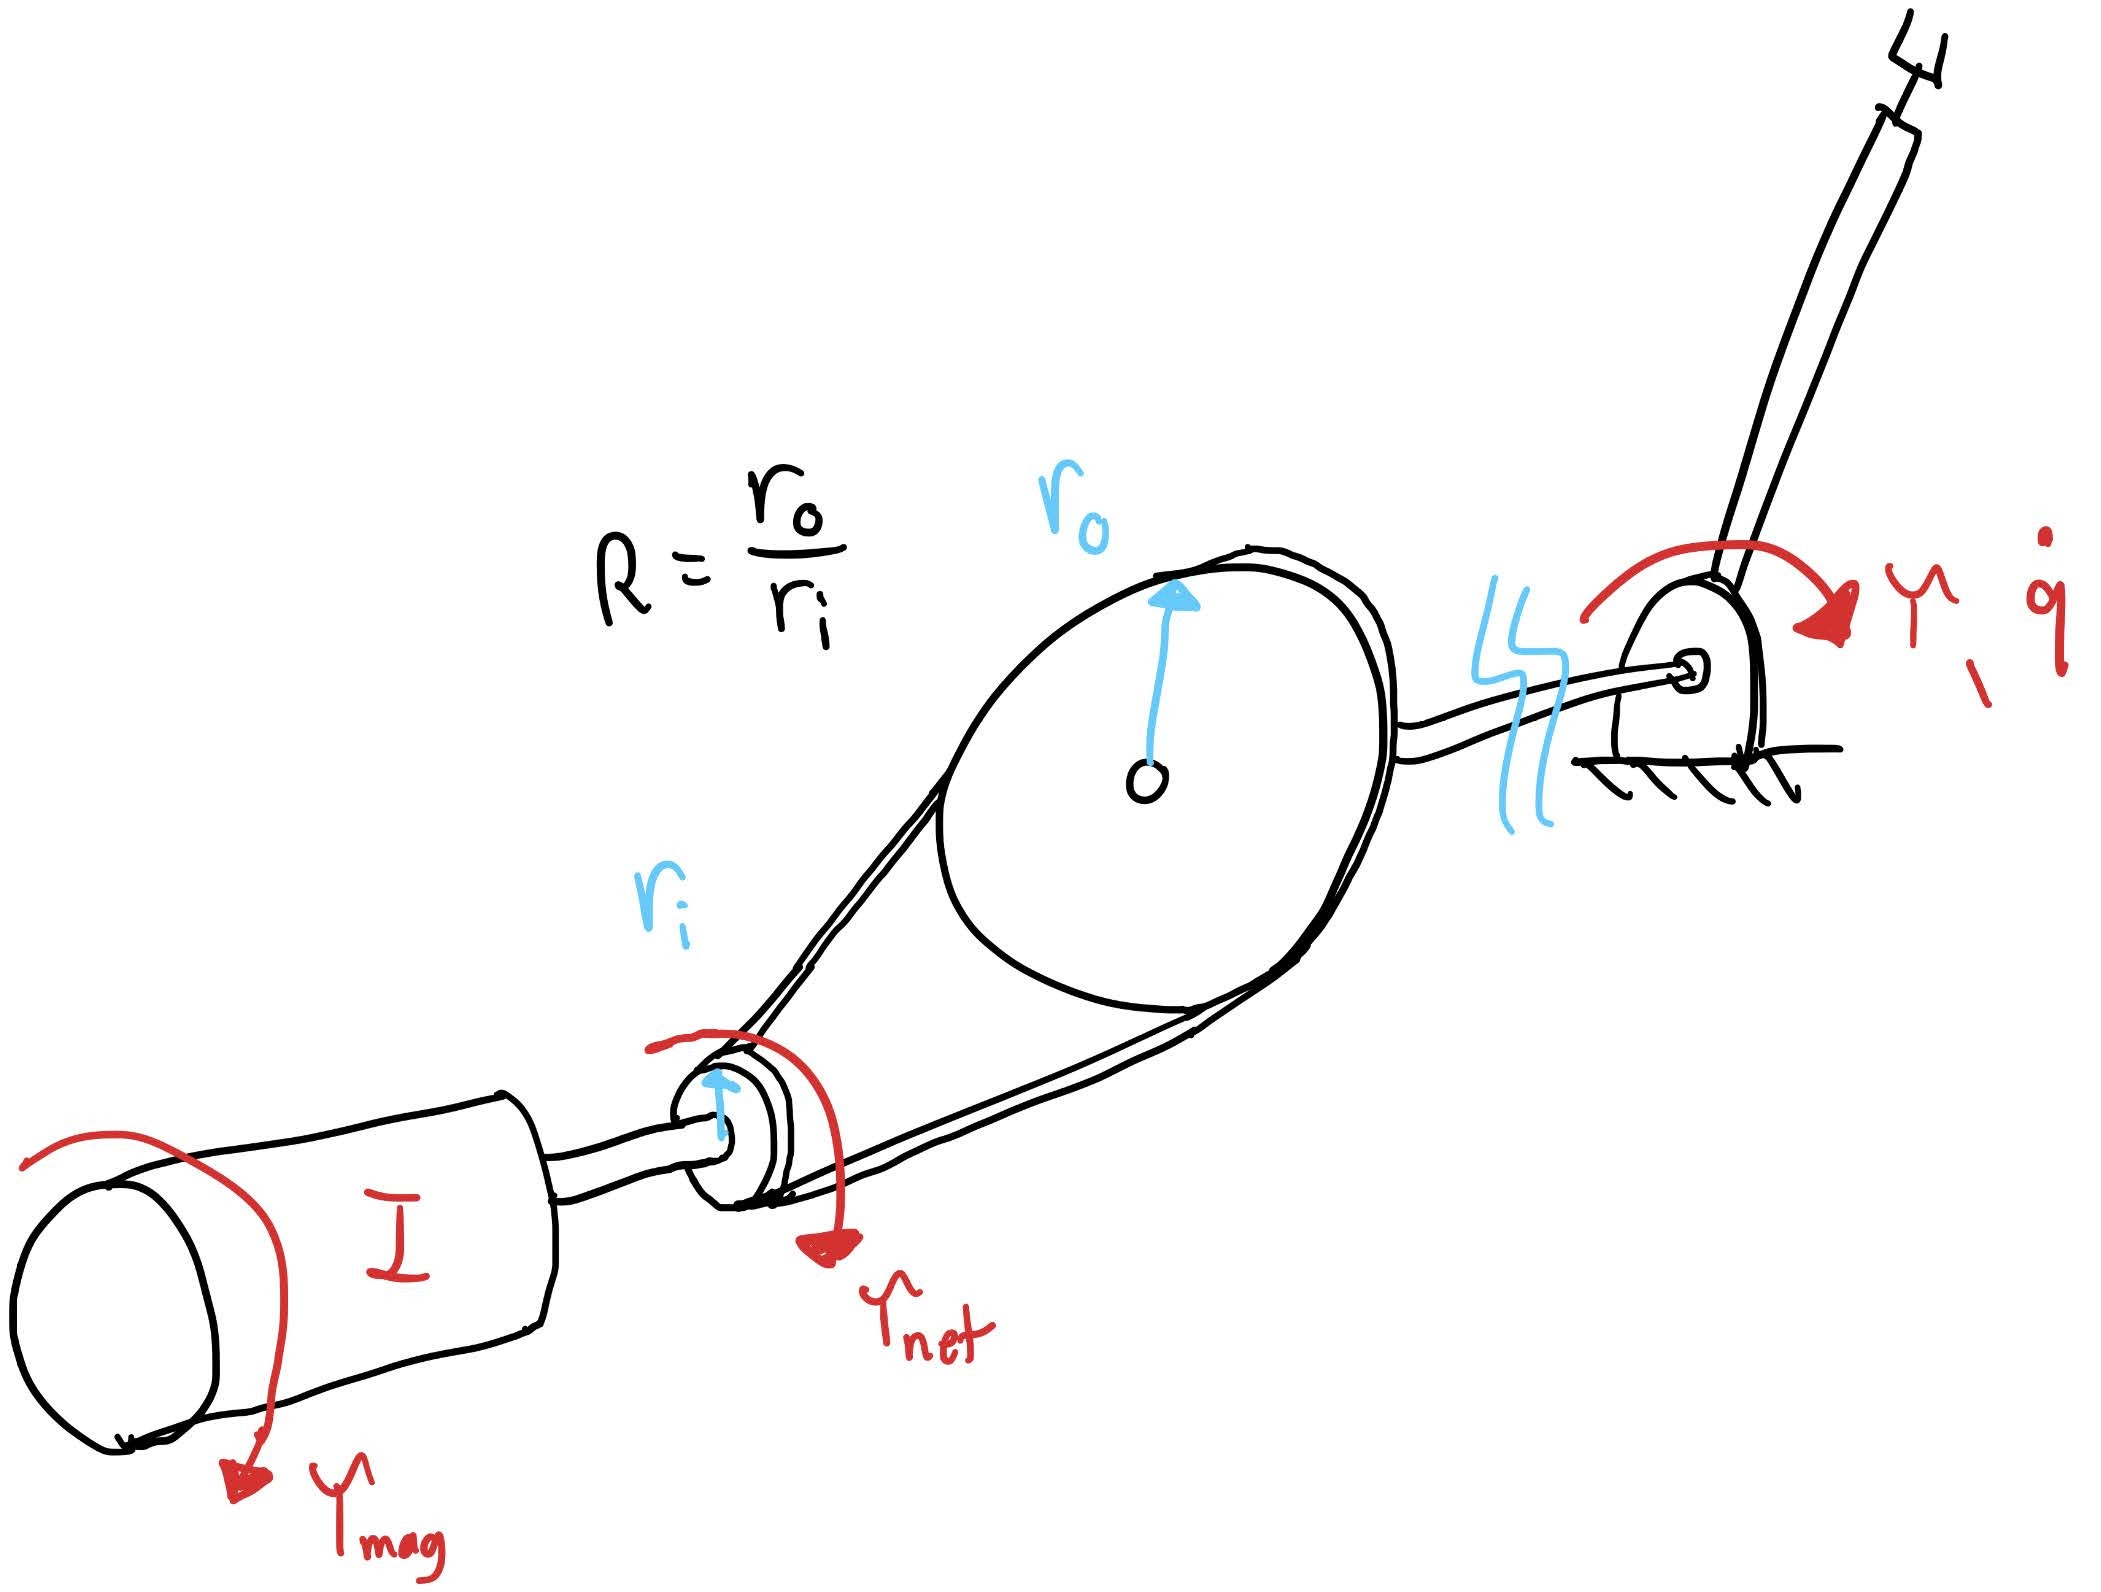
\includegraphics[width=0.70\textwidth]{fig/actuator_dynamic.jpg}
	\caption{Dynamique d'un moteur électrique couplé avec un joint robotique}%
	\label{fig:actuator_dynamic}
\end{figure}
%%%%%%%%%%%%%%%%%%%%%%%%%%%%%%%%%%%%%%%%%%%%%%%%%%%%%%%%%%%%%%%%%%%%%%%%%%%%











% BACKUP ENG

\iftoggle{EN}{%
\section{Equations of motion in joint-space}
%\section{Équations du mouvement dans l'espace des joints}
\label{sec:eom}

The general form of the equations of motion of robotic systems (interconnected rigid body driven by motors) is:
%
\begin{align}
H(\col{q}) \col{\ddot{q}} + C(\col{q},\col{\dot{q}}) \col{\dot{q}} + D \col{\dot{q}} + \col{g}(\col{q}) = B(\col{q}) \col{\tau} 
\label{eq:manipulator}
\end{align}
%
where $\col{q}$ is the generalized coordinates vector, $H$ is the inertia matrix, $C$ is the Coriolis/centrifugal force matrix, $D$ is a damping matrix, $\col{g}$ is the gravitational forces vector and $B$ is a matrix mapping motor torques $\col{\tau}$ into generalized forces.
%
Kinetic energy is given by:
%
\begin{align}
\frac{1}{2} \col{\dot{q}}^T H(\col{q}) \col{\dot{q}} 
\label{eq:kinetic}
\end{align}
%
Conservation of energy also give the following relation:
%
\begin{align}
\dot{H} = C + C^T
\label{eq:cener}
\end{align}
%
On occasion, dependence notation is dropped and $\col{h}$ is used to represent all state dependent forces, leading to the short form:
%
\begin{align}
H \col{\ddot{q}} + \col{h} = B \col{\tau} 
\label{eq:manipulator_short}
\end{align}

\begin{table}[htbp]
	\centering
	\caption{Nomenclature pour la dynamique dans l'espace des joints}	% Table caption must be placed on top of the table %
		\begin{tabular}{ c c l r }
        \hline \hline
				\multicolumn{4}{c}{Scalars} \\
				\hline \hline
			$n$             &  :  & number of DoF                                              & \\
			$m$             &  :  & number of actuators                                        & \\
			$c$             &  :  & number of contact constraints                              & \\
			$o$             &  :  & number of end-effector coordinates                         & \\ 
			$i$             &  :  & index for DoF                                              & \\ 
			\hline \hline
			\multicolumn{4}{c}{Vectors} \\
			\hline \hline
			$\col{\tau}$    &  :  & Actuator forces/torques                                    & $m$  \\
			$\col{q}$       &  :  & Joint coordinates position vector                          & $n$  \\
			$\col{w}$       &  :  & Actuator coordinates velocity vector                          & $m$  \\ 
			$\col{g}$       &  :  & Gravitational forces vector                                & $n$  \\
			$\col{h}$       &  :  & Sum of state-dependent generalized forces                  & $n$  \\
			$\col{\phi}$    &  :  & Constraint vector                                          & $c$  \\
			$\col{f}_C$     &  :  & Contact forces vector                                      & $c$  \\
			$\col{f}_e$     &  :  & End-effector external forces vector                        & $o$  \\
			$\col{r}$       &  :  & End-effector position vector                               & $o$  \\
			\hline \hline
			\multicolumn{4}{c}{Matrices} \\
			\hline \hline
			$H$             &  :  & Inertia matrix                                             & $n$ x $n$ \\
			$D$             &  :  & Damping matrix                                             & $n$ x $n$ \\
			$C$             &  :  & Coriolis/Centrifugal forces matrix                         & $n$ x $n$ \\
			$B$             &  :  & Generalized forces matrix                                  & $n$ x $m$ \\
			$J_a$           &  :  & Actuator coordinates / joint coordinates Jacobian matrix   & $m$ x $n$ \\
			$J_e$           &  :  & Task-space coordinates / joint coordinates Jacobian matrix & $o$ x $n$ \\
			$J_C$           &  :  & Contact constraints Jacobian matrix                        & $c$ x $n$  \\
		\hline \hline
        \end{tabular}		
	\label{tab:nom}
\end{table}




Fig. \ref{fig:coord} shows all the used coordinates systems. 
%
\begin{figure}[H]
	\centering
		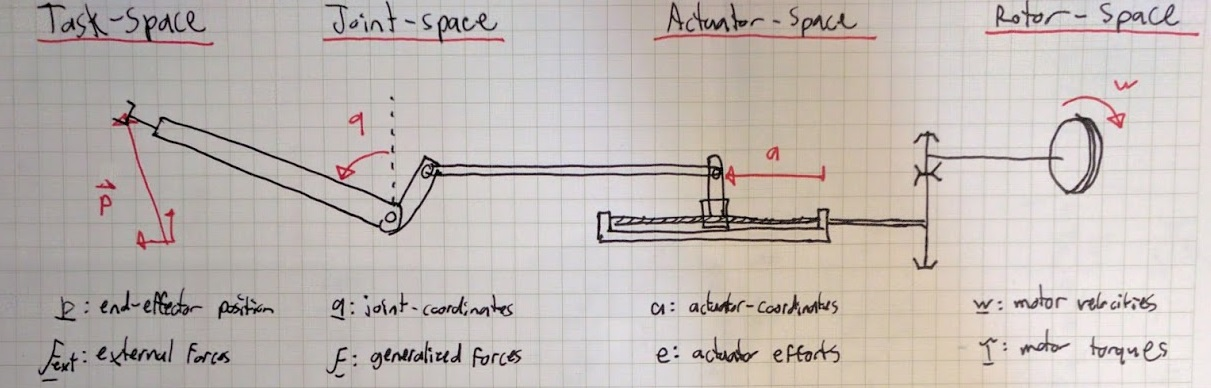
\includegraphics[width=0.99\textwidth]{coord.jpg}
	\caption{Coordinate systems}%
	\label{fig:coord}
\end{figure}
%
Where coordinates transforms are defined by:
%
\begin{align}
\col{\dot{r}}   &= J_e( \col{q} ) \col{\dot{q} }  \quad \text{ from joint-space to end-effector   } \\
\col{\dot{a}}   &= J_a( \col{q} ) \col{\dot{q} }  \quad \text{ from joint-space to actuator-space } \\
\col{w }        &= R              \col{\dot{a} }  \quad\quad \text{ from actuator-space to rotor-space } 
\label{eq:coord_transform2}
\end{align}
%
%
The following equation represents the most general case:
%
\begin{align}
H \col{\ddot{q}} + C \col{\dot{q}} + D \col{\dot{q}} + \col{g} =  \underbrace{ J_a^T(\col{q}) R^T }_{B(\col{q})}  \col{\tau} + J_e^T(\col{q}) \col{f}_e + J_C^T(\col{q}) \col{f}_C
\label{eq:manipulator_gen}
\end{align}


\newpage
\section{Contact}
\label{sec:contact}

This section presents equations for representing contact situations.

\subsubsection{Kinematic constraints}
\label{sec:constraints}
%
If a robotic manipulator enter contact with a fixed object, then some DoF are constrained. In the case of a bilateral constraint, the constraint can be expressed as:
\begin{align}
\col{\phi}( \col{ q } ) = 0
\label{eq:constraint}
\end{align}
%
The time-derivative of the constraint must also be equal to zero, which gives some constraints in terms of velocity and acceleration:
\begin{align}
\frac{d \col{\phi}( \col{ q } ) }{dt}     &= J_C( \col{ q } ) \col{\dot{q}}  = 0 \\
\frac{d^2 \col{\phi}( \col{ q } ) }{dt^2} &= J_C( \col{ q } ) \col{\ddot{q}}  + \dot{J}_C( \col{ q } ) \col{\dot{q}} = 0 
\label{eq:constraint_diff}
\end{align}
%
when $J_C$ is the constraint Jacobian:
%
\begin{align}
J_C( \col{ q } )                    &= \frac{d \col{\phi}( \col{ q } ) }{d\col{ q }}
\label{eq:constraint_jaco}
\end{align}

\subsubsection{Constraint forces}
\label{sec:constraint_forces}

The constraint Jacobian can be used to map constraint forces $\col{f}_C$ to generalized forces in the EoM:
%
\begin{align}
H \col{\ddot{q}} + \col{h} = B \col{\tau} + J_C( \col{ q } )^T  \col{f}_C
\label{eq:manipulator_constraint}
\end{align}
%
Solving for $\col{\ddot{q}}$ in eq. \eqref{eq:manipulator_constraint} and substituting in eq. \eqref{eq:constraint_diff}, it is possible to get and expression for the constraint forces $\col{f}_C$ as a function of states and applied torques:
%
\begin{align}
\col{f}_C = \left( J_C H^{-1} J_C^T \right)^{-1} \left(  J_C H^{-1} [\col{h} - B \col{\tau} ] - \dot{J}_C( \col{ q } ) \col{\dot{q}}   \right)
\label{eq:const_forces}
\end{align}
%
Alternatively, it possible to solve for acceleration $\col{\ddot{q}}$ and constraints forces $\col{f}_C$ simultaneously by solving the following system of equations:
%
\begin{align}
\left[ \begin{array}{c c } 	H & -J_C^T  \\ J_C 	& 0  	\end{array} \right] \left[ \begin{array}{c} \col{\ddot{q}}  \\ \col{f}_C \end{array} \right] = \left[ \begin{array}{c}  B \col{\tau} - \col{h}   \\ -\dot{J}_C \col{\dot{q}}  \end{array} \right]
\label{eq:manipulator_constraint_eom}
\end{align}


\subsubsection{Impact impulsive behavior}
\label{sec:impact}
%
When the robot first enters contact with a fixed object, impulsive contact forces will act on the system. Integrating eq. \eqref{eq:manipulator_constraint} over the short impact interval gives:
%
\begin{align}
\int{ ( H \col{\ddot{q}} + \col{h} ) dt } &= \int{ ( B \col{\tau} + J_C( \col{ q } )^T  \col{f}_C ) dt } \\
H \col{\dot{q}}^+ - H \col{\dot{q}}^- &= J_C( \col{ q } )^T  \int{  \col{f}_C dt }
\label{eq:manipulator_impact}
\end{align}
%
where any non-impulsive forces are neglected during the short impact interval. Projecting onto constrained coordinates (multiplying by $J_C H^{-1}$) gives:
%
\begin{align}
J_C \col{\dot{q}}^+ - J_C \col{\dot{q}}^- &= J_C H^{-1} J_C^T  \int{  \col{f}_C dt }
\label{eq:manipulator_impact2}
\end{align}
%
Then assuming a sticky inelastic impact (no bouncing), then the constraint is respected after the impact ($J_C \col{\dot{q}}^+=0$) and it is possible to solve for the impact force:
%
\begin{align}
\int{  \col{f}_C dt } &= - \left( J_C H^{-1} J_C^T \right)^{-1}  J_C \col{\dot{q}}^-
\label{eq:manipulator_impact_force}
\end{align}
%
and also for the velocity after the impact:
%
\begin{align}
\col{\dot{q}}^+ &= - \Big[ I - H^{-1} J_C^T \left( J_C H^{-1} J_C^T \right)^{-1} J_C \Big] \col{\dot{q}}^-
\label{eq:manipulator_impact_velocity}
\end{align}
%
Or change in velocity:
%
\begin{align}
\Delta \col{\dot{q}} &=  \Big[ H^{-1} J_C^T \left( J_C H^{-1} J_C^T \right)^{-1} J_C \Big] \col{\dot{q}}^-
\label{eq:manipulator_impact_velocity_delta}
\end{align}
%

Alternatively, it possible to solve for velocity $\col{\dot{q}}^+$ and impulsive forces $\int{ \col{f}_C dt }$ simultaneously by solving the following system of $n+c$ equations:
%
\begin{align}
\left[ \begin{array}{c c } 	H & -J_C^T  \\ J_C 	& 0  	\end{array} \right] \left[ \begin{array}{c} \col{\dot{q}}^+  \\ \int{ \col{f}_C dt }\end{array} \right] = \left[ \begin{array}{c}  	H \col{\dot{q}}^-   \\ 0  \end{array} \right]
\label{eq:manipulator_impact_eom}
\end{align}


\section{Hybrid system dynamics}

Hybrid dynamical system can be represented in the general form:
%
\begin{align}
\text{Continuous evolution: } \left(  \dot{\col{x}} , \dot{k} \right) &=  \left( \, f_k( \col{x} , \col{u} , \col{d} ) \, , \, 0 \, \right) \\
\text{Discrete jumps: } \left(  \col{x}^+ , k^+ \right) &=  \left( h_{ij}( \col{x}^- , \col{u}^- ) , j \right) \quad\text{if}\quad \left(  \col{x} , k , \col{u} \right) \in D_{ij}  
\end{align}
%
where $\col{x}$ is a continuous state vector, and $k$ is a discrete mode and $D_{ij}$ is the domain mapping conditions leading to a transition $k:i \rightarrow j$. For robotic systems, the discrete mode can represent discrete configurations of the robot , like discrete modes in the control law or contact/non-contact conditions. The jump map then represents the impulsive response when contact is made. 

\subsection{Switched system}

A restricted class of hybrid system, called switched system, are hybrid systems for which the jump map for continuous state is the identify function:
%
\begin{align}
\text{Continuous evolution: } \left(  \dot{\col{x}} , \dot{k} \right) &=  \left( \, f_k( \col{x} , \col{u} , \col{d} ) \, , \, 0 \, \right) \\
\text{Discrete jumps: } \left(  \col{x}^+ , k^+ \right) &=  \left( \col{x}^- , j \right) \quad\text{if}\quad \left(  \col{x} , k , \col{u} \right) \in D_{ij} 
\end{align}
%

\subsubsection{Switched system where the discrete mode is a control input}

In the situation where the discrete operating mode $k$ is a control input, then there is no need to keep track of discrete mode evolution and only the piece-wise continuous differential equations are sufficient to model the system evolution:
%
\begin{align}
\dot{\col{x}} = f_k( \col{x} , \col{u} , \col{d} ) 
\end{align}
%
A robot with a continuous dynamics but with a control law using discrete modes of operation would be of this category. 


}{}